%% =====================================================================
%%  Towards Longitudinal Prediction of Parkinson's Disease Motor Subtypes
%%  Preprint source.  Compile with:  pdflatex -> bibtex -> pdflatex x2
%% =====================================================================
\documentclass[11pt]{article}

\usepackage[T1]{fontenc}
\usepackage[utf8]{inputenc}
\usepackage{amsmath,amssymb}
\let\Bbbk\relax
\usepackage{newtxtext,newtxmath}
\usepackage[margin=1.15in]{geometry}
\usepackage{graphicx}
\usepackage{booktabs}
\usepackage{array}
\usepackage{authblk}
\usepackage[numbers,sort&compress]{natbib}
\usepackage{microtype}
\usepackage{url}
\usepackage[font=small,labelfont=bf,width=.95\textwidth]{caption}
\usepackage{fancyhdr}
\usepackage[hidelinks]{hyperref}

\graphicspath{{figures/}}

\renewcommand{\arraystretch}{1.08}
\setlength{\parskip}{0pt}
\setlength{\skip\footins}{14pt}

\pagestyle{fancy}
\fancyhf{}
\renewcommand{\headrulewidth}{0pt}
\fancyfoot[C]{\thepage}

\newcommand{\TD}{\mathrm{TD}}
\newcommand{\PIGD}{\mathrm{PIGD}}
\newcommand{\Ind}{\mathrm{Ind}}

\title{\bfseries Towards Longitudinal Prediction of\\
Parkinson's Disease Motor Subtypes}

\author[1]{Parv Patel}
\author[1]{Mayank Tewatia}
\author[2]{Varsha Vasudevan}
\author[1]{K.~R.~Sahasranand}
\affil[1]{\normalsize Indian Institute of Technology Palakkad, India}
\affil[2]{\normalsize NeuroComp}

\date{}

\begin{document}
\maketitle
\thispagestyle{fancy}

\begin{abstract}
\noindent
Parkinson's disease is commonly divided into tremor-dominant (TD) and postural
instability and gait difficulty (PIGD) motor subtypes, with an Indeterminate
band between them. The subtype is obtained by thresholding the ratio of two
averages of MDS-UPDRS items, and a change of subtype over time is widely treated
as a marker of motor progression. Much modelling work therefore aims to predict
this label, but the reliability of the label itself is rarely measured first. We
ask whether longitudinal prediction of the motor subtype is limited by the
choice of model family, or by the label being predicted. Using the Parkinson's
Progression Markers Initiative observational cohort --- 1,080 patients and 4,441
labelled visits, of which 934 patients with two or more labelled visits
contribute 3,361 consecutive visit-to-visit transitions --- we applied one
evaluation protocol to four model families: discrete-time and continuous-time
Markov chains on the observed label; a hidden Markov model (HMM) with a latent
state and a fitted misclassification matrix; a hierarchical Bayesian growth
model on the ratio; and Gaussian process (GP) regression on the ratio and on the
tremor and PIGD subscores. Every model was evaluated by leave-one-patient-out
validation with patient-clustered bootstrap intervals. The recorded label is
unstable: 35.2\% of observed subtype changes revert at the very next visit, and
requiring a conversion to hold for two consecutive assessments removes 51.7\% of
apparent PIGD conversions. Held-out three-class accuracy over the same 3,361
transitions was 0.7539 (95\% CI 0.7348--0.7731) for the HMM, 0.7474 and 0.7453
for the two observed-label chains, 0.7227 for a persistence rule that simply
repeats the current subtype, and 0.6293 for a marginal null. The best
discrete-state model therefore gains $+3.1$ accuracy points (95\% CI $+2.2$ to
$+4.1$) over persistence, and it assigns the Indeterminate class once in 3,361
opportunities. The hierarchical Bayesian model estimates a population trend of
$-0.093$ per year in the ratio (95\% credible interval $-0.116$ to $-0.068$)
against a total residual spread of 1.14 --- about 4.6 times the width of the
Indeterminate band --- so the middle class is nearly unreachable for any model
that predicts the band from a continuous quantity. On the ratio, a GP with a
flexible kernel improves on a linear-trend GP ($-0.033$ mean absolute error,
95\% CI $-0.047$ to $-0.021$); but modelled separately, the GP did not beat
persistence on the tremor subscore and was worse on the PIGD subscore.
Converting the subscore GP predictions back to a subtype permits a like-for-like
comparison with the HMM on exactly the same 934 patients and 3,361 points: GP-derived
accuracy was 75.66\% against the HMM's 75.39\%, a paired difference of
$+0.27$ points (95\% CI $-0.42$ to $+0.98$). Four families embodying
substantially different assumptions thus converge on the same held-out
performance, a few points above a trivial rule, and none recovers the
Indeterminate class. With frequent label reversion and a residual spread several
times the band width, this points to the representation of motor symptoms,
rather than model capacity, as the binding constraint. The target is the next
recorded output of a labelling rule, not an independent clinical diagnosis; the
matched comparison is a failure to detect a difference and does not establish
equivalence; no external cohort was used and no clinical utility is claimed.
\end{abstract}

\medskip
\noindent\textbf{Keywords:} Parkinson's disease; motor subtype; tremor dominant;
postural instability and gait difficulty; longitudinal prediction; label
reliability; hidden Markov model; Gaussian process; PPMI.

% =====================================================================
\section{Introduction}
% =====================================================================

Parkinson's disease is clinically heterogeneous, and the most widely used
summary of that heterogeneity in motor terms divides patients into a
tremor-dominant (TD) group, a postural instability and gait difficulty (PIGD)
group, and an Indeterminate group between them. In the MDS-UPDRS era the
division is operational rather than mechanistic: eleven items are averaged into
a tremor score, five into a PIGD score, and the ratio of the two is compared
against a pair of thresholds, with the interval between them forming the
Indeterminate band~\citep{stebbins2013,goetz2008}. The rule is cheap to apply,
interpretable, and computable from an examination that is performed anyway,
which is why it is distributed as a derived variable and why most longitudinal
studies of subtype stability have used it.

The label is used well beyond description. It stratifies cohorts, defines
subgroups for biomarker comparison, and is increasingly treated as a prediction
target in its own right: a model is trained on a patient's history and asked
what subtype will be recorded at the next visit. A change of subtype over time
is then read as a marker of motor progression.

Three claims are easy to conflate here, and this paper keeps them apart
throughout. Predicting a \emph{recorded subtype label} is predicting the output
of a deterministic rule applied to sixteen ratings at a future examination.
Predicting \emph{underlying motor progression} is a statement about a patient's
phenotype. Predicting an \emph{independent clinical diagnosis} is a statement
about an adjudicated assessment that this rule does not provide. These are not
equivalent, and only the first is the target of the models evaluated here.

Several groups have shown that the recorded label moves. Substantial fractions
of de novo patients change subtype within twelve months~\citep{simuni2016},
comparable instability has been reported over three years in an independent
early-disease cohort~\citep{kohat2021}, and competing subtyping algorithms
applied to the same patients agree only fairly with one
another~\citep{ren2020,ren2021}. What this literature establishes is that the
label \emph{changes}. What it does not establish is \emph{why} --- and the
distinction matters for anyone training a model on it. Stability studies measure
change as a comparison between a baseline and a later assessment, or as a shift
in prevalence across a cohort. That design cannot separate a patient whose
phenotype genuinely progressed from one whose single noisy assessment crossed a
threshold and crossed back, because both appear as a changed subtype. Separating
them requires three consecutive assessments and a statistic that asks how often
a change is undone.

A second gap concerns how predictive studies of this endpoint are reported.
Discrimination is reported far more often than
calibration~\citep{vancalster2019}, and we are not aware of a study of subtype
prediction that reports what a trivial rule --- naming the currently recorded
label --- achieves on the same evaluation set. Without that comparison, an
accuracy figure on a label this persistent is hard to interpret, because a
target whose majority class repeats at better than 80\% rewards a model for
doing nothing.

The natural response to a hard prediction problem is a larger model. Before
assuming that more capacity will help, it is worth asking whether the ceiling is
a property of the model or of the measurement. That is the question of this
paper:

\begin{quote}
\emph{Is longitudinal prediction of the Parkinson's disease motor subtype
limited more by model capacity, or by the reliability and representation of the
subtype labels themselves?}
\end{quote}

\subsection*{Contributions}

\begin{enumerate}
\itemsep2pt
\item \textbf{A reliability characterisation of the endpoint, measured before
any model is fitted.} We quantify how often an observed subtype change is undone
at the next visit, how the conversion incidence depends on whether a change is
required to be sustained, how transition probabilities scale with the elapsed
interval, and whether the recorded label satisfies the first-order Markov
property.

\item \textbf{A comparison of four model families under one protocol.}
Observed-label Markov chains, a latent-state hidden Markov model with an
explicit misclassification matrix, a hierarchical Bayesian growth model on the
ratio, and Gaussian processes on the ratio and on the two subscores are scored
on one common set of 3,361 held-out prediction opportunities, under one decision
rule, one patient-clustered bootstrap, and one parameter-free baseline.

\item \textbf{A quantitative account of why the Indeterminate class is not
recovered.} The growth model's posterior gives a residual spread for the ratio
that is about 4.6 times the width of the Indeterminate band, and the attainable
values of the ratio inside that band are few and concentrated at its edges. The
two facts together explain a negative result that every family in the comparison
shares.

\item \textbf{A matched cross-family comparison.} Converting continuous subscore
predictions back through the unchanged classification rule allows a Gaussian
process and a hidden Markov model to be compared on exactly the same patients
and prediction points. We report the paired difference and its interval, and we
state explicitly that failing to detect a difference is not evidence of
equivalence.
\end{enumerate}

This study proposes no new model. Its unit of contribution is a set of
measurements about an endpoint, and a protocol under which claims about that
endpoint can be compared.

% =====================================================================
\section{Related Work}
% =====================================================================

\paragraph{Motor subtype classification.}
The TD/PIGD division used here follows the MDS-UPDRS adaptation of
\citet{stebbins2013}, derived from the scale of \citet{goetz2008}. An
international appraisal of Parkinson's disease subtype classifications examined
many such systems and found the supporting evidence base thin, noting in
particular that longitudinal stability had not been assessed for most of
them~\citep{mestre2021}; a subsequent purpose-driven framework recommends asking
what a subtype is \emph{for} before asking whether it is real~\citep{marras2024}.
Whether the PIGD construct identifies a distinct phenotype at all, rather than a
stage of disease, has been questioned separately~\citep{nutt2016,urso2022}.

\paragraph{Stability of the label over follow-up.}
\citet{simuni2016} reported the baseline distribution and one-year instability of
the classification in the de novo PPMI cohort. \citet{kohat2021} followed
MDS-UPDRS subtypes over three years in an independent early-disease cohort.
\citet{ren2020,ren2021} compared three published subtyping algorithms in the same
de novo patients and found only fair agreement between them. These studies
measure net drift between assessments. None reports, to our knowledge, the
proportion of observed changes that are reversed at the next assessment --- the
statistic that distinguishes phenotypic progression from assessment variability,
and the one we report in Section~\ref{sec:stability}.

\paragraph{Longitudinal progression modelling in Parkinson's disease.}
\citet{severson2021} learned latent disease states from many clinical
measurements in PPMI using an input--output hidden Markov model, and
\citet{fereshtehnejad2017} derived clinical subtyping criteria with longitudinal
validation. Both target \emph{data-driven} states rather than the published
threshold rule, so their results do not bear directly on the predictability of
that rule's output. Multistate Markov models that treat a recorded state as a
noisy reading of a latent one, through an explicit misclassification matrix, are
long established in panel-data analysis~\citep{jackson2011}; we use that
construction as one of four families rather than as a proposed method.
Hierarchical Bayesian growth models and Gaussian process
regression~\citep{rasmussen2006} are standard tools for individual longitudinal
trajectories, and we apply them to the continuous quantity from which the label
is cut.

\paragraph{Benchmarking practice.}
\citet{vancalster2019} document how rarely clinical prediction models are
reported with calibration alongside discrimination, and proper scoring rules
provide the principled alternative to thresholded
accuracy~\citep{gneiting2007}. Our protocol applies both, and adds the element
we found missing throughout this literature: a parameter-free baseline evaluated
on the identical case list, with paired intervals.

\paragraph{How this study differs.}
Prior work establishes that the label changes and that competing definitions
disagree. This study measures the label's reliability in a way that separates
reversion from progression, then asks four dissimilar model families the same
prediction question on one case list, and uses the agreement among them --- and
their shared failure on one class --- as evidence about the target rather than
about any one model.

% =====================================================================
\section{Data and Cohort}
\label{sec:data}
% =====================================================================

\subsection{Data source}
Data came from the Parkinson's Progression Markers Initiative
(PPMI)~\citep{marek2011ppmi}, an ongoing international observational study.
Three sources were used: the PPMI Curated Data Cut (public release 2026-05-11),
which supplies the visit skeleton and covariates; the item-level MDS-UPDRS Part
II (patient questionnaire) and Part III (motor examination) files, which supply
the sixteen ratings from which the subtype is derived; and the participant
status file.

\subsection{Cohort definition}
Participants were included if the curated cut assigned them to the sporadic
Parkinson's disease subgroup. Visits were excluded if they were unscheduled or
premature-withdrawal encounters, or if they fell beyond fifteen years of
follow-up. Of 4,788 participants and 19,450 visits in the curated cut, 1,080
participants contributing 5,774 visits met these criteria
(Figure~\ref{fig:flow}).

A motor subtype could be assigned at 4,441 of those visits (76.9\%). Of the
1,080 participants, 934 had at least two labelled visits and therefore
contributed at least one prediction opportunity; these patients account for
4,295 labelled visits and \textbf{3,361 consecutive labelled visit pairs}, which
form the evaluation set used throughout. Cohort characteristics are given in
Table~\ref{tab:cohort}. At the first labelled visit, 772 participants (71.7\%)
were tremor dominant, 109 (10.1\%) Indeterminate and 195 (18.1\%) PIGD, within
one percentage point in each class of an independent analysis of the same
cohort~\citep{simuni2016}. The median interval between consecutive labelled
visits was 1.00 years and the median follow-up 3.1 years.

\begin{figure}[t]
\centering
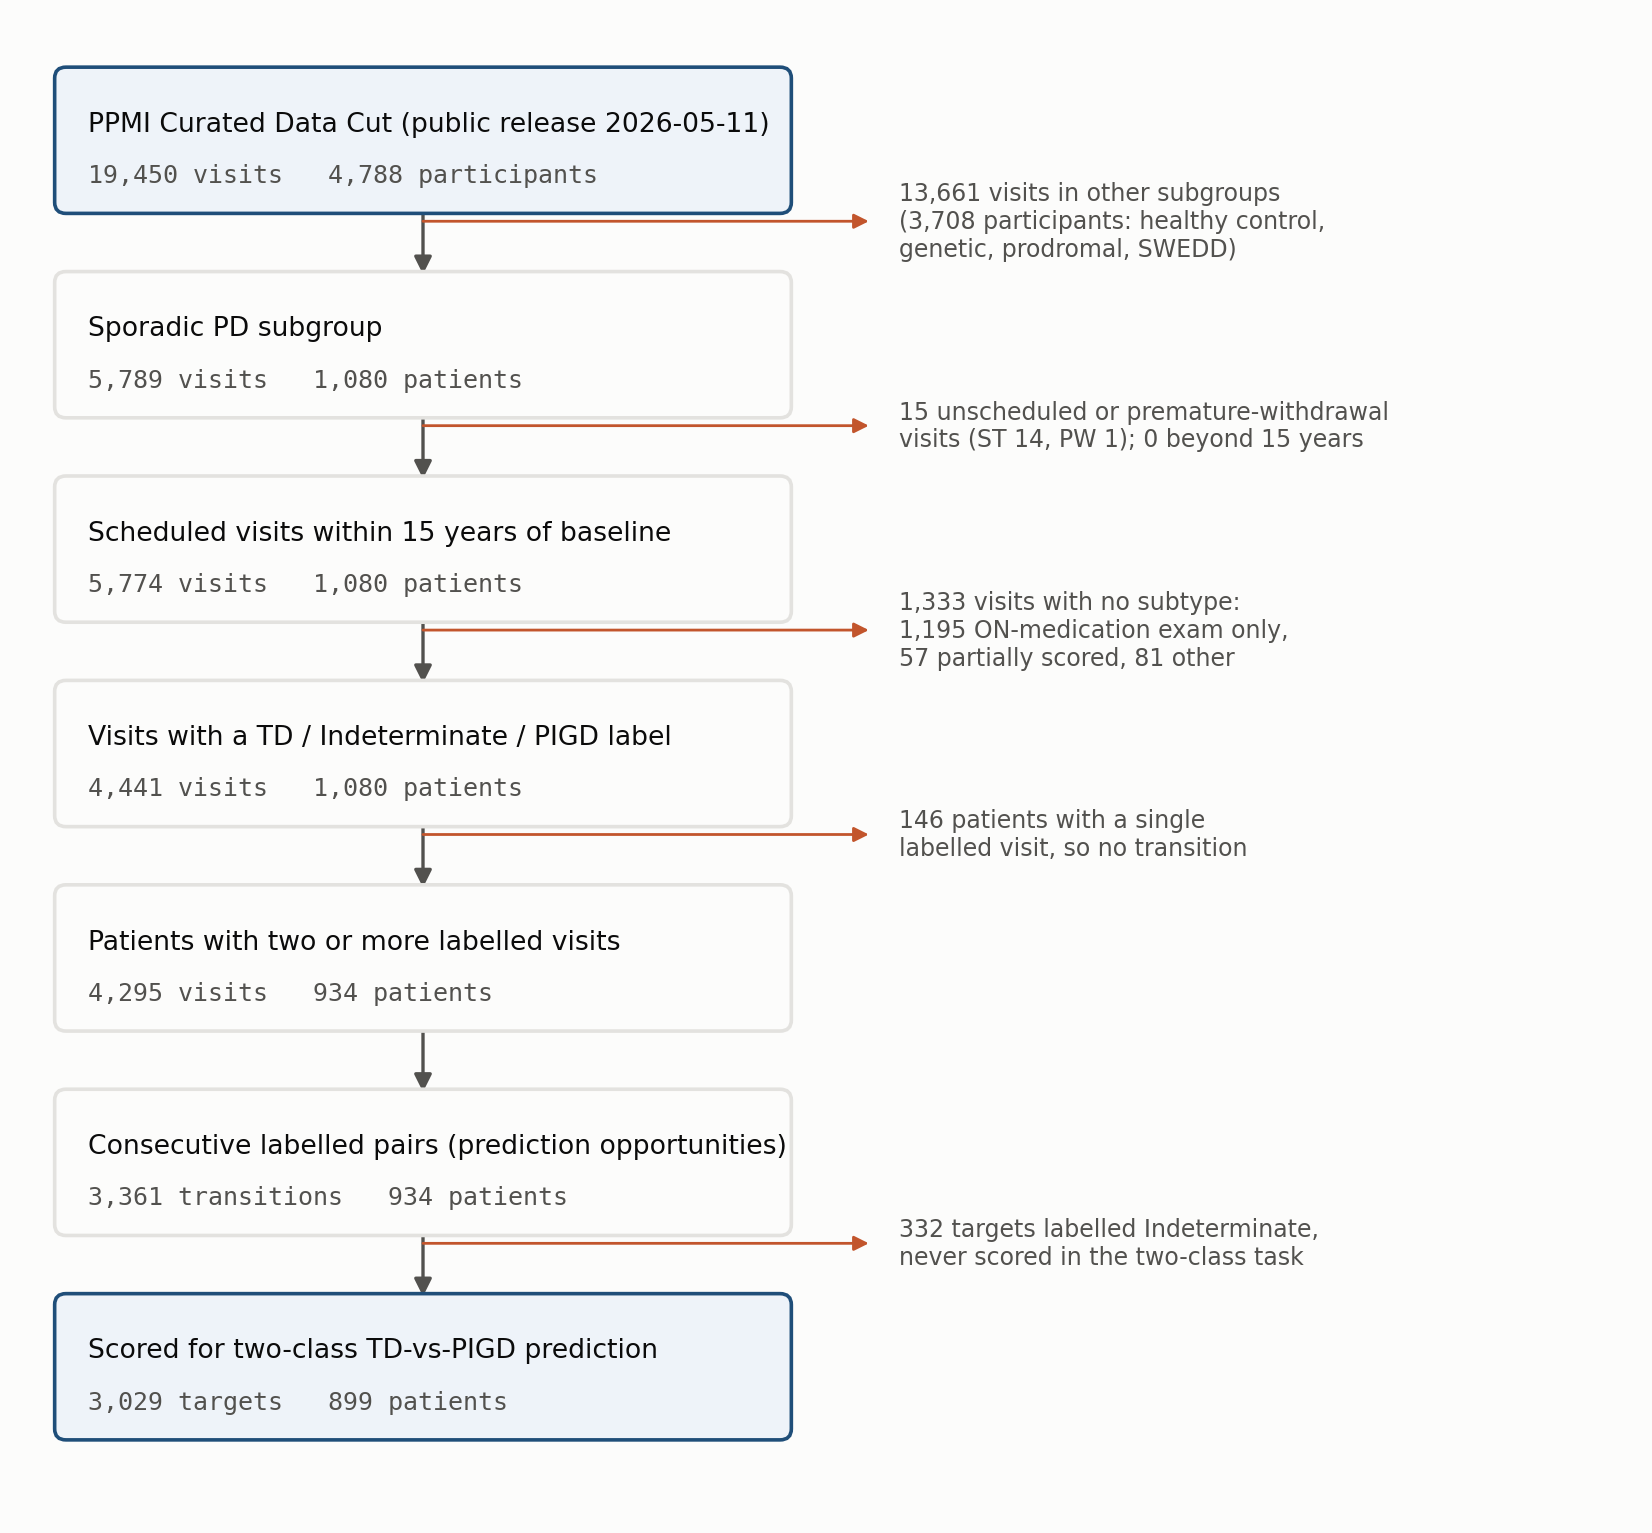
\includegraphics[width=0.84\textwidth]{fig1_flow.png}
\caption{Participant flow from the curated data cut to the evaluation set, with
every exclusion counted. The dominant cause of label loss is the OFF-medication
requirement rather than an incomplete examination: 1,195 of 1,333 unlabelled
visits (89.6\%) carried only an ON-medication Part III examination. The final
box is the two-class evaluation set used in secondary analyses; the three-class
analyses reported here use the 3,361 transitions of the box above it.}
\label{fig:flow}
\end{figure}

\begin{table}[t]
\centering
\caption{Cohort characteristics. Continuous variables are measured at the
participant's first visit and reported as median (interquartile range). The
subtype distribution at the first visit is over the 1,076 first visits that
carry a label. The modelling cohort is the subset of patients contributing at
least one visit-to-visit transition.}
\label{tab:cohort}
\small
\begin{tabular}{@{}lrr@{}}
\toprule
 & Full cohort & Modelling cohort \\
Characteristic & ($\geq 1$ labelled visit) & ($\geq 2$ labelled visits) \\
\midrule
Patients, $n$                              & 1,080 & 934 \\
Labelled visits, $n$                       & 4,441 & 4,295 \\
Labelled visits per patient                & 3 (2--5) & 4 (3--6) \\
Follow-up, y                               & 3.0 (1.4--5.1) & 3.1 (2.1--6.9) \\
Interval between labelled visits, y        & \multicolumn{2}{c}{1.00 (1.00--1.16)} \\
\addlinespace[2pt]
Male, $n$ (\%)                             & 709 (65.6) & 615 (65.8) \\
Age at baseline, y                         & 64.1 (57.1--70.1) & 63.8 (56.8--69.7) \\
Education, y                               & 16 (14--18) & 16 (14--18) \\
Disease duration at baseline, y            & 0.5 (0.3--1.0) & 0.5 (0.3--1.0) \\
Hoehn \& Yahr stage                        & 2.0 (1.0--2.0) & 2.0 (1.0--2.0) \\
MDS-UPDRS Part II                          & 5 (3--9) & 5 (3--9) \\
MDS-UPDRS Part III (OFF)                   & 21 (15--28) & 21 (15--28) \\
MoCA                                       & 27 (26--29) & 27 (26--29) \\
\addlinespace[2pt]
Tremor subscore (11 items)                 & 0.5 (0.3--0.8) & 0.5 (0.3--0.8) \\
PIGD subscore (5 items)                    & 0.2 (0.0--0.4) & 0.2 (0.0--0.4) \\
Ratio $r$, where defined                   & 1.8 (0.9--2.7) & 1.8 (0.9--2.8) \\
Visits with $r$ undefined ($P=0$), $n$ (\%) & 725 (16.3) & 692 (16.1) \\
\midrule
\multicolumn{3}{@{}l}{\textit{Subtype at the first labelled visit}} \\
\quad Tremor dominant                      & 772 (71.7\%) & 676 (72.5\%) \\
\quad Indeterminate                        & 109 (10.1\%) & 99 (10.6\%) \\
\quad PIGD                                 & 195 (18.1\%) & 157 (16.8\%) \\
\addlinespace[2pt]
\multicolumn{3}{@{}l}{\textit{Subtype over all labelled visits}} \\
\quad Tremor dominant                      & 2,891 (65.1\%) & --- \\
\quad Indeterminate                        & 441 (9.9\%) & --- \\
\quad PIGD                                 & 1,109 (25.0\%) & --- \\
\bottomrule
\end{tabular}

\end{table}

\subsection{Subtype labels and the MDS-UPDRS components}
\label{sec:labels}
The \emph{tremor score} $T$ is the mean of eleven MDS-UPDRS items (2.10;
3.15a--b; 3.16a--b; 3.17a--e; 3.18) and the \emph{PIGD score} $P$ the mean of
five (2.12, 2.13, 3.10, 3.11, 3.12), following \citet{stebbins2013}. The
classification rule applied to $r = T/P$ is given in Section~\ref{sec:rule}.

Three data-handling decisions materially affect the result and are stated in
full. First, PPMI records ``unable to rate'' as the sentinel value 101 \emph{in
the same numeric field as a valid 0--4 rating}; every value outside the valid
range was blanked before any mean was taken. This is not a rounding concern: one
such value among the five PIGD items lifts their mean to roughly 20 and
reclassifies a tremor-dominant visit as PIGD. Second, a subscore was set to
missing if \emph{any} constituent item was missing, matching PPMI's own
derivation. Third, the classification uses the \emph{OFF-medication or
untreated} examination, because levodopa suppresses tremor and scoring
ON-state examinations would manufacture apparent PIGD transitions that are
pharmacological rather than pathological. Where a visit carried more than one
eligible Part III examination, the record with the fewest missing items was
retained.

Recomputed labels were validated against PPMI's own two derivations: agreement
was 4,431 of 4,431 (100.00\%) against the curated cut's two-class label, and
1,595 of 1,597 (99.87\%) against a three-class label in an archived release
covering 390 participants.

\subsection{Missingness and exclusions}
Labels were not imputed; all analyses used complete cases. Of the 1,333 cohort
visits without a subtype, 1,195 (89.6\%) had only an ON-medication Part III
examination and were excluded by the medication-state rule; 65 had no Part III
record; 57 had an examination that was recorded but incomplete; and 16 had a
complete Part III but an incomplete Part II. The dominant mechanism is therefore
treatment-related, and the loss is not random: unlabelled visits came
overwhelmingly from treated participants later in follow-up (median 5.0 years
from baseline against 2.0; 96.8\% on antiparkinsonian medication against
57.9\%). The analysed sample is consequently weighted towards earlier, untreated
follow-up, which attenuates rather than exaggerates observed progression.

\subsection{Visits at which the ratio is undefined}
\label{sec:undefined}
The ratio $r = T/P$ is undefined when $P = 0$. Among all 4,441 labelled visits
this occurs at \textbf{725 visits (16.3\%)}; among the 4,295 labelled visits
contributed by the 934 patients of the modelling cohort it occurs at
\textbf{692 visits (16.1\%)}. These visits are overwhelmingly tremor dominant:
of the 725, 665 are TD (a patient with some tremor and no recorded postural or
gait impairment) and 60 are the doubly degenerate case $T = P = 0$, classified
Indeterminate.

This matters for the interpretation of every analysis in this paper that models
the ratio. The hierarchical Bayesian growth model and the ratio Gaussian process
are defined on $r$ and therefore cannot use these visits at all, whereas the
Markov models, the hidden Markov model and the subscore Gaussian processes
retain them. \textbf{The ratio-based subset is not a random subset of the
cohort}: it systematically excludes the most strongly tremor-dominant
assessments, so quantities estimated on it are conditioned on the presence of
some postural or gait impairment and should not be read as cohort-wide. Where a
comparison spans a ratio model and a non-ratio model, we restrict it to the
transitions both can score and say so.

% =====================================================================
\section{Methods}
% =====================================================================

\subsection{Motor subtype definition}
\label{sec:rule}
Writing $T$ and $P$ for the tremor and PIGD means of Section~\ref{sec:labels}
and $r = T/P$, the subtype at a visit is
\begin{equation}
\mathrm{subtype} =
\begin{cases}
\TD,   & r \geq 1.15 \ \text{ or } (P = 0,\ T > 0),\\[2pt]
\PIGD, & r \leq 0.90,\\[2pt]
\Ind,  & \text{otherwise.}
\end{cases}
\label{eq:rule}
\end{equation}
The final branch covers $0.90 < r < 1.15$ and the doubly degenerate case
$T = P = 0$. The band is open at both ends, so a ratio falling exactly on a
threshold is assigned to the outer class, and the two degenerate cases are
handled explicitly rather than by division.

Two properties of this definition are relevant throughout. First, the
Indeterminate band is only $0.25$ wide on a quantity whose observed values span
$0$ to $11.4$. Second, because $T$ is a mean of eleven integer ratings and $P$ a
mean of five, $r$ takes values on a lattice rather than a continuum, and very
few lattice points fall inside a band that narrow. Both are measured in
Section~\ref{sec:ind}.

\subsection{Longitudinal prediction task}
\label{sec:task}
Visits were ordered within patient by elapsed time from that patient's first
visit. Unlabelled visits were removed before pairing, so a missing year does not
break a sequence; a \emph{transition} is a pair of consecutive \emph{labelled}
visits, carrying the actual elapsed interval between them.

The task is: given a patient's history up to and including visit $k$, and the
elapsed interval $\Delta$ to visit $k+1$, predict the subtype recorded at visit
$k+1$. The unit of prediction is one transition, and the evaluation set is the
3,361 transitions of Section~\ref{sec:data}.

What is available at prediction time is the patient's own labelled history
$y_1,\dots,y_k$ (or, for the continuous models, the subscore or ratio history),
the elapsed times between those visits, and the interval $\Delta$ to the target
visit. The model is told \emph{when} the next visit happens, not what is
recorded at it. This is the usual convention for panel data but is an assumption
worth stating: no result here addresses when a patient will next be seen, and
all transition probabilities are conditional on the next visit occurring.

\subsection{Observed-label Markov models}
Two specifications treat the recorded label itself as the state, so that the
state space is $\mathcal{S} = \{\TD, \Ind, \PIGD\}$ and no latent structure is
posited.

The \emph{discrete-time chain} estimates a row-stochastic matrix $A$ with
$A_{ab} = \Pr(y_{k+1} = b \mid y_k = a)$ from the observed pairs by maximum
likelihood, ignoring the elapsed interval. Its assumption is that the next label
depends on the current one and on nothing else, including the time between
visits.

The \emph{continuous-time chain} relaxes the second half of that assumption. It
estimates a generator $Q$ with non-negative off-diagonal entries and rows
summing to zero, giving
\begin{equation}
\Pr(y_{k+1} = b \mid y_k = a,\ \Delta) = \bigl[\exp(Q\Delta)\bigr]_{ab},
\label{eq:ctmc}
\end{equation}
where $\exp(\cdot)$ is the matrix exponential. Off-diagonal rates are
parameterised as $\exp(\theta)$ to keep them positive. This specification is
interval-aware but still first-order in the observed label.

Whether that first-order assumption holds is testable without fitting either
model, by asking whether the next label is conditionally independent of the
previous one given the current one. We test this on consecutive triples with a
$\chi^2$ test of independence, separately for each current state
(Section~\ref{sec:stability}).

\subsection{Hidden Markov model}
\label{sec:hmm}
The hidden Markov model separates what is recorded from what is modelled as
evolving. A latent state $X(t) \in \mathcal{S}$ evolves as a continuous-time
Markov chain with generator $Q$, and what is observed at visit $k$ is not
$X(t_k)$ but a noisy reading $Y_k$ related to it by a misclassification matrix
$E$,
\begin{equation}
E_{ab} = \Pr(Y_k = b \mid X(t_k) = a), \qquad \sum_b E_{ab} = 1 .
\label{eq:emission}
\end{equation}
The likelihood of one patient's whole sequence marginalises over every latent
path by the forward algorithm,
\begin{equation}
L = \pi^{\!\top} \! \operatorname{diag}(E_{\cdot y_1})
    \prod_{k=2}^{K} \exp\!\bigl(Q \Delta_{k-1}\bigr)
    \operatorname{diag}(E_{\cdot y_k})\, \mathbf{1},
\label{eq:forward}
\end{equation}
and a prediction for visit $k+1$ is obtained by filtering the history to a
posterior over $X(t_k)$, propagating it through $\exp(Q\Delta)$, and passing it
through $E$. Specifications with three and five latent states were fitted by
maximum likelihood with deterministic restarts.

A constraint is required. Left unconstrained, the maximum-likelihood solution is
degenerate and identical across random restarts: the latent Indeterminate state
emits uniformly and PIGD becomes absorbing at the parameter boundary. We
therefore require each state to be recorded correctly more often than not,
$E_{aa} \geq 0.5$. The fitted diagonal was 0.941 for TD and 0.842 for PIGD; for
Indeterminate it sat exactly at the floor of 0.500, which is a result about that
state rather than an artefact of the constraint.

The latent states of this model are a modelling device. They are estimated
solely from the sequence of recorded labels and their timings, and nothing in
this design identifies them with clinically validated phenotypes. We refer to
them as latent states throughout and do not interpret them as independently
confirmed subtypes.

\subsection{Hierarchical Bayesian growth model}
\label{sec:hb}
The growth model abandons the discrete label and models the continuous quantity
the label is cut from. For patient $i$ at time $t_{ij}$ years from that
patient's first visit,
\begin{align}
r_{ij} &= \bigl(\beta_0 + b_{0i}\bigr) + \bigl(\beta_1 + b_{1i}\bigr) t_{ij} + \varepsilon_{ij},
\label{eq:hb}\\[2pt]
b_{0i} &\sim \mathcal{N}(0, \tau_0^2), \quad
b_{1i} \sim \mathcal{N}(0, \tau_1^2), \quad
\varepsilon_{ij} \sim \mathcal{N}(0, \sigma^2),
\nonumber
\end{align}
with $\beta_0, \beta_1$ the population intercept and slope, $b_{0i}, b_{1i}$
patient-level deviations, and $\varepsilon_{ij}$ residual variation. The model
was fitted by Gibbs sampling under weakly informative priors.

Two points of specification matter. First, $\sigma$ is the \emph{total} residual
SD. Separate observation and process terms, both additive on the same
observation, are not separately identifiable, so only their sum is estimated.
Second, the model is defined on $r$ and therefore uses only visits at which $r$
is defined (Section~\ref{sec:undefined}); it was fitted on 2,426 observations
from 573 training patients.

A subtype prediction is derived by applying the unchanged
rule~\eqref{eq:rule} to the predictive distribution of $r$. This makes the
relationship between the residual spread $\sigma$ and the width of the
Indeterminate band directly interpretable, and we report it in
Section~\ref{sec:hbres}.

\subsection{Gaussian process models}
\label{sec:gp}
Gaussian process regression~\citep{rasmussen2006} replaces the parametric linear
trend of~\eqref{eq:hb} with a distribution over functions. For a patient's
trajectory $f(t)$ we take $f \sim \mathcal{GP}\bigl(m(t), k(t,t')\bigr)$ with a
fitted linear mean function $m(t)$ and Gaussian observation noise, and compare
four covariance functions:
\begin{align*}
K_0:&\quad k = \sigma_c^2 + \sigma_\ell^2\, t t'  &&\text{(constant + linear)}\\
K_1:&\quad k = \sigma_c^2 + \sigma_f^2 \exp\!\bigl(-\tfrac{(t-t')^2}{2\ell^2}\bigr) &&\text{(constant + squared exponential)}\\
K_2:&\quad k = \sigma_c^2 + \sigma_\ell^2\, t t' + \sigma_f^2 \exp\!\bigl(-\tfrac{(t-t')^2}{2\ell^2}\bigr) &&\text{(both)}\\
K_3:&\quad k = \sigma_c^2 + \sigma_\ell^2\, t t' + \text{Mat\'ern-}3/2 &&\text{(rougher alternative)}
\end{align*}
$K_0$ is the Gaussian process analogue of a linear trend and is the natural
comparator for the growth model; $K_1$ is the flexible alternative. The
comparison $K_1$ versus $K_0$ asks whether departures from a straight line carry
predictive signal, and $K_3$ versus $K_1$ asks whether the trajectory is rougher
than a squared-exponential kernel allows.

Gaussian processes were fitted to three targets: the ratio $r$, and the tremor
and PIGD subscores modelled separately. The subscore models were additionally
fitted in a jointly-covarying form, in which the two subscores share a
covariance so that their predictions are correlated.

Subtype predictions were derived from the subscore models by pushing the
predictive distribution through the project's own unchanged classification
function by Monte Carlo: 10,000 draws per case from the model's joint predictive
distribution over $(T, P)$, each draw classified by~\eqref{eq:rule}, and the
resulting class frequencies taken as the three-class probability vector. Common
random numbers were used across specifications so that draws cancel in paired
contrasts. Halving the number of draws moved accuracy by at most 0.0015 for any
specification, and the vectorised implementation of~\eqref{eq:rule} was checked
against the reference implementation on 5,000 synthetic cases including 400
both-subscores-zero and 600 PIGD-zero cases (5,000 of 5,000 agreement).

The Gaussian process predicts subscores and, through~\eqref{eq:rule}, the label
derived from them. It does not predict clinical disease progression directly,
and no result in Section~\ref{sec:gpres} should be read as doing so.

\subsection{Patient-level validation}
\label{sec:validation}
All models were validated by \textbf{leave-one-patient-out} cross-validation.
For each of the 934 patients in turn, the model is refitted from scratch on all
other patients and then used to predict that patient's recorded subtypes one
visit at a time. \emph{No visit of the held-out patient enters the fit}, and
each prediction uses only that patient's own earlier visits as history. This
yields 3,361 held-out predictions from 934 patients for every specification, and
it is the same case list for every specification.

The structural point is that the holdout is at the level of the \emph{patient},
not the visit. Because one patient contributes several correlated transitions,
holding out a visit while training on its neighbours from the same patient would
leak information; holding out the patient removes that channel entirely.

A battery of ten checks was asserted at run time on every saved prediction row:
that every patient is held out exactly once; that the held-out patient is the
patient being predicted; that every fold trained on all other patients; that the
prediction count equals the transition count; that the history is strictly the
visits before the target; that the target visit is always later than the current
visit; that probabilities sum to one; that the predicted class is the argmax;
that the confusion-matrix totals equal the prediction count; and that every fit
converged. All ten passed for the three-state specifications.

The hierarchical Bayesian growth model and the ratio Gaussian process are
defined on the ratio and so cannot score every transition. Where they are
compared against a model that can, the comparison is restricted to the
transitions both can score, and the restricted sample size is reported with the
result.

\subsection{Evaluation metrics and statistical analysis}
\label{sec:stats}
The central methodological step in comparing families is that \textbf{every
specification is expressed as a three-class predictive probability vector over
$(\TD, \Ind, \PIGD)$ on the same 3,361 cases, and the predicted class is the
argmax of that vector}. The chains and the hidden Markov models are natively on
this representation; the continuous models are converted as described in
Section~\ref{sec:gp}. No tuned thresholds and no per-model calibration are
applied.

This harmonisation is not cosmetic. The same saved predictions from one Gaussian
process score 0.7298 under a point-estimate label derivation and 0.7566 under
the probability-vector derivation --- a difference larger than the entire spread
between the fitted specifications.

Models are compared on accuracy, multiclass Brier score, log loss, macro-F1 and
per-class recall. Accuracy alone is reported nowhere without a probabilistic
companion~\citep{gneiting2007,vancalster2019}, because on a three-class target
with a small middle class the two can rank specifications in opposite orders.
Continuous targets are scored by mean absolute error (MAE), root mean squared
error, continuous ranked probability score (CRPS) and the coverage of the stated
95\% predictive interval. Because the subscores and the ratio are non-negative
while the models place Gaussian predictive distributions on them, we also report
the predictive mass falling below zero as a diagnostic of misspecification.

\paragraph{Uncertainty.}
Because one patient contributes several correlated transitions, every interval
reported here is a \textbf{patient-level cluster bootstrap}: patients are drawn
with replacement carrying all of their visits, and every statistic is recomputed
from scratch in each replicate. Paired contrasts share one resample between the
two conditions in every replicate, so the reported difference and its interval
are paired. Intervals from the hierarchical Bayesian model are \emph{credible}
intervals from the posterior and are labelled as such; all others are bootstrap
\emph{confidence} intervals, and the two are not interchangeable.

\paragraph{Interpretation of intervals.}
We report whether an interval excludes zero, which is a statement about
precision, and separately whether a difference is large enough to matter, which
is not. An interval that contains zero is a \emph{failure to detect} a
difference at this sample size; it is not evidence that two models are
equivalent, and we do not treat it as such anywhere in this paper. Multiplicity
is largely uncorrected across the specifications compared, and analyses
described as exploratory were specified after the predictions were generated.

% =====================================================================
\section{Results}
% =====================================================================

\subsection{The recorded label is unstable, and a third of the change reverses}
\label{sec:stability}

Across the 3,361 transitions, TD was the most persistent recorded state and
Indeterminate by far the least (Figure~\ref{fig:instability}a,
Table~\ref{tab:transitions}). A visit recorded TD was followed by another TD
visit with probability 0.808 (95\% CI 0.788--0.826), and a PIGD visit by another
PIGD visit with probability 0.702 (0.661--0.738). A visit recorded Indeterminate
remained Indeterminate with probability only 0.192 (0.148--0.234), returning to
TD in 0.440 (0.381--0.500) of cases and moving to PIGD in 0.368 (0.318--0.417).
PIGD was not absorbing: 29.8\% of PIGD visits were followed by a non-PIGD
assessment.

\begin{figure}[t]
\centering
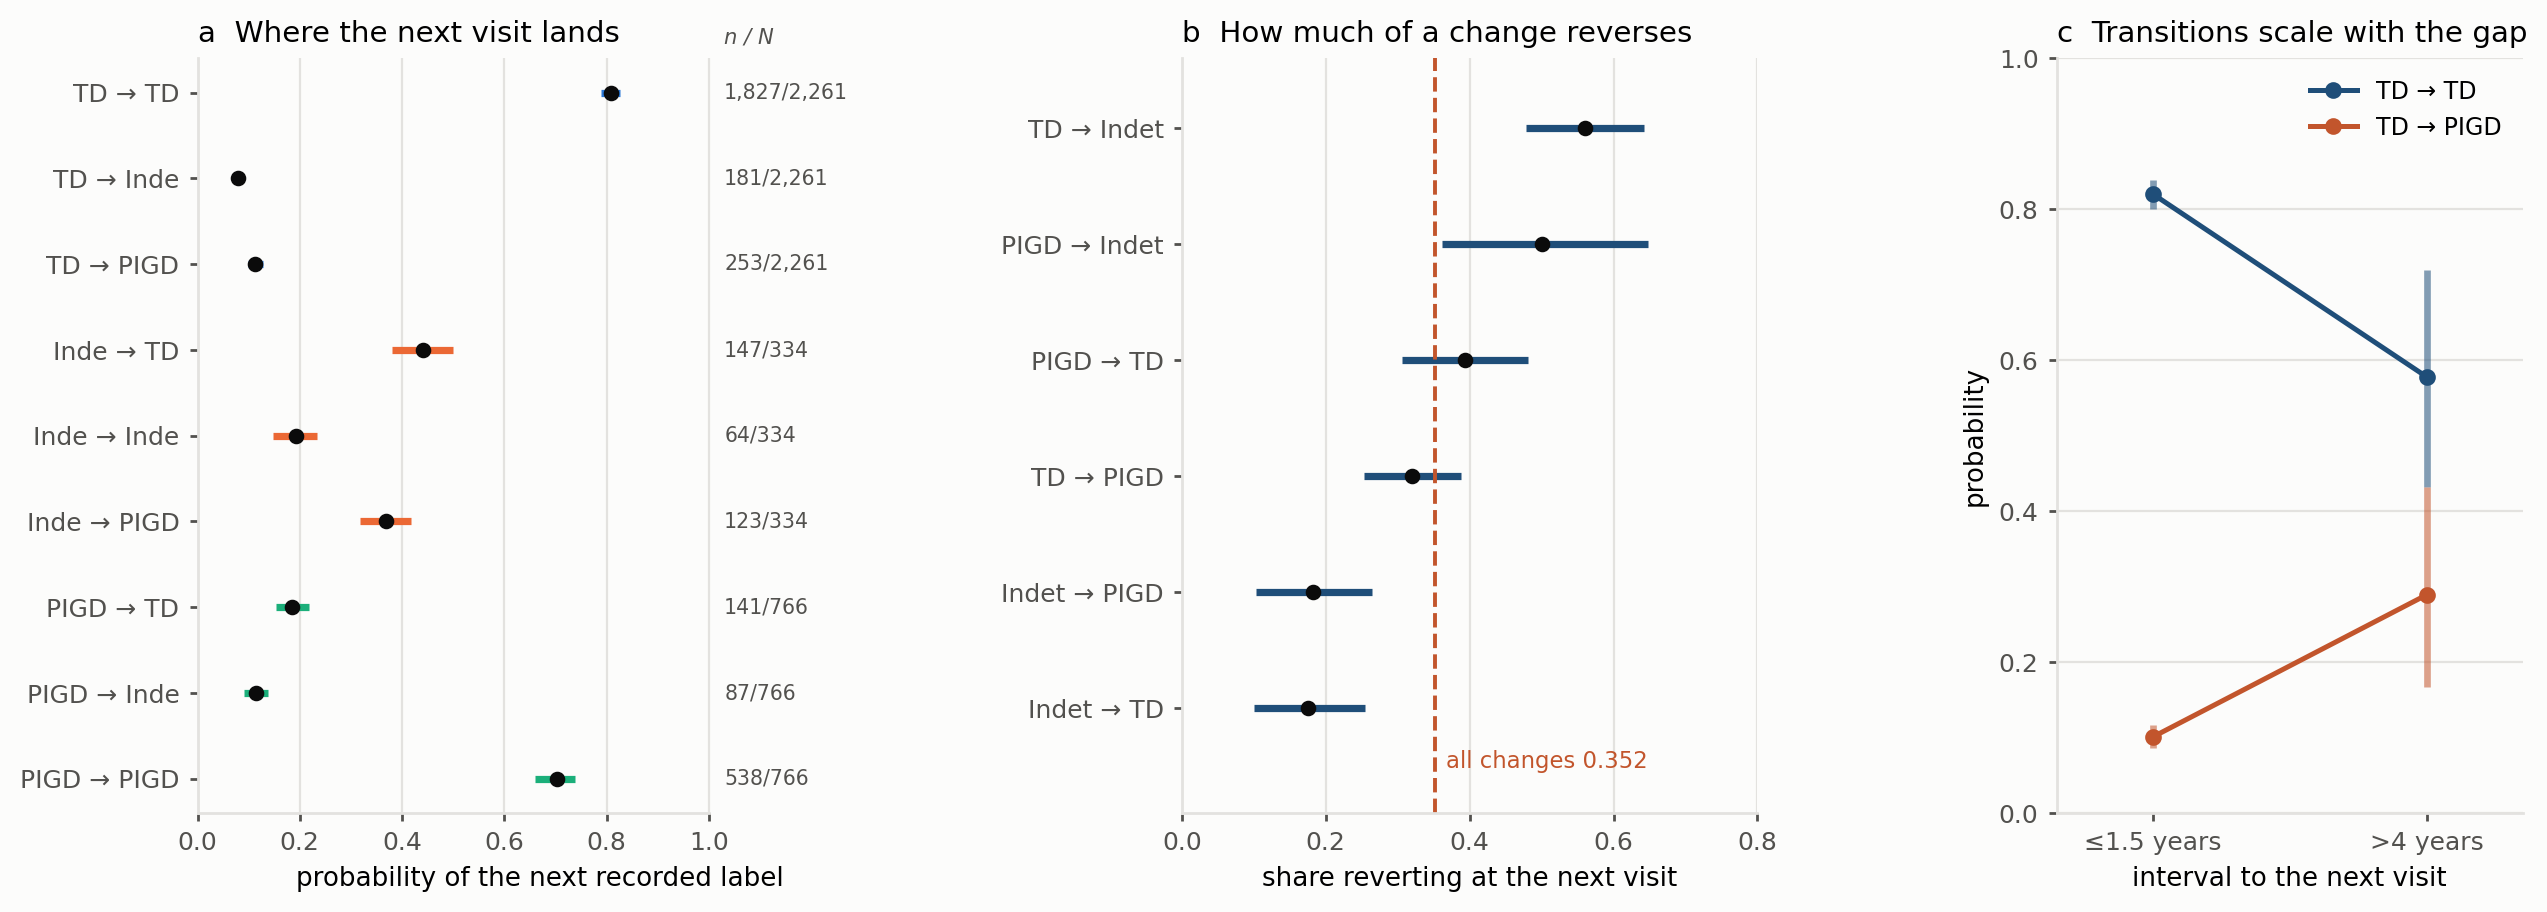
\includegraphics[width=\textwidth]{fig2_instability.png}
\caption{The recorded label is unstable, and much of the instability is not
progression. (\textbf{a}) One-step transition probabilities over the 3,361
consecutive labelled visit pairs, with patient-clustered bootstrap 95\%
intervals; the $x$-axis is the probability of each next recorded label and the
counts at the right are the numerator and denominator of each estimate.
(\textbf{b}) Of every observed change of state, the proportion back at the
origin state one visit later, with the pooled rate of 0.352 marked; changes into
the Indeterminate band revert far more often than changes crossing the full
width of the scale. (\textbf{c}) TD$\to$TD and TD$\to$PIGD probabilities
stratified by the elapsed interval to the next visit, showing that a single
pooled transition matrix averages intervals that behave differently.}
\label{fig:instability}
\end{figure}

\begin{table}[t]
\centering
\caption{One-step transition probabilities between consecutive labelled visits,
with patient-clustered bootstrap 95\% intervals over the 934 patients. Rows sum
to one.}
\label{tab:transitions}
\small
\begin{tabular}{@{}llrrl@{}}
\toprule
Subtype at visit $k$ & Subtype at visit $k+1$ & $n$ & $\hat{p}$ & 95\% CI \\
\midrule
TD ($n{=}2{,}261$) & TD & 1,827 & 0.808 & (0.788, 0.826) \\
 & Indeterminate & 181 & 0.080 & (0.068, 0.092) \\
 & PIGD & 253 & 0.112 & (0.098, 0.127) \\
\addlinespace[2pt]
Indeterminate ($n{=}334$) & TD & 147 & 0.440 & (0.381, 0.500) \\
 & Indeterminate & 64 & 0.192 & (0.148, 0.234) \\
 & PIGD & 123 & 0.368 & (0.318, 0.417) \\
\addlinespace[2pt]
PIGD ($n{=}766$) & TD & 141 & 0.184 & (0.153, 0.218) \\
 & Indeterminate & 87 & 0.114 & (0.091, 0.138) \\
 & PIGD & 538 & 0.702 & (0.661, 0.738) \\
\bottomrule
\end{tabular}

\end{table}

\paragraph{A third of observed changes reversed immediately.}
Of 673 observed changes of state, \textbf{35.2\% (31.8--38.8) returned to the
origin state at the following visit} (Figure~\ref{fig:instability}b). Reversion
was concentrated in changes involving the Indeterminate band: TD$\to$Indeterminate
reversed in 0.560 (0.478--0.642) of cases and PIGD$\to$Indeterminate in 0.500
(0.362--0.648), while changes crossing the full width of the scale reversed less
often --- TD$\to$PIGD in 0.320 (0.253--0.388) and PIGD$\to$TD in 0.393
(0.305--0.481).

This is the statistic that separates the two readings of an observed change. A
change that is undone at the very next assessment is not easily read as
phenotypic progression, and more than a third of changes in this cohort were.

\paragraph{The definition of a conversion dominates its estimated frequency.}
Among the 885 patients not PIGD at their first labelled visit, 263 converted to
PIGD on a single-assessment definition but only 127 when the conversion was
required to hold across two consecutive labelled visits --- a reduction of
\textbf{51.7\% (45.7--57.7)}. Kaplan--Meier cumulative incidence at five years
was 35.3\% (30.8--39.9) under the single-visit definition against 15.3\%
(12.0--19.0) under the sustained one. The two definitions differ by roughly a
factor of two on the same patients.

\paragraph{Transition probabilities scale with the elapsed interval.}
TD$\to$TD fell from 0.820 at intervals of 1.5 years or less to 0.578 beyond four
years, while TD$\to$PIGD rose from 0.100 to 0.289
(Figure~\ref{fig:instability}c), the two interval-stratified intervals being
non-overlapping. A single pooled matrix therefore averages one-year and
multi-year transitions in whatever proportion attendance happened to produce,
and is not a property of the disease. This motivates the interval-aware
specifications of~\eqref{eq:ctmc} and~\eqref{eq:forward}.

\paragraph{The observed label is not first-order Markov.}
Testing whether the next label is conditionally independent of the previous one
given the current one rejects independence in all three current states: for
current TD, $\chi^2 = 156.59$ on 4 degrees of freedom over 1,583 triples
($p = 7.9 \times 10^{-33}$); for current Indeterminate, $\chi^2 = 15.28$ over
235 triples ($p = 0.0042$); for current PIGD, $\chi^2 = 61.15$ over 609 triples
($p = 1.7 \times 10^{-12}$). Concretely, among currently-TD patients the
probability of a PIGD outcome was 0.086 if the previous label had been TD and
0.393 if it had been PIGD.

The correct reading is that the current recorded label is not a sufficient
statistic for the past. This motivates a latent-state formulation, in which a
slower underlying state carries the history that the recorded label does not,
but it does not by itself establish one: unequal visit intervals and
within-patient correlation could also produce history dependence, and the test
treats triples as independent when patients contribute several.

\subsection{Discrete-state models: four families converge a few points above a trivial rule}
\label{sec:discrete}

Under one decision rule, one evaluation set and one baseline, the discrete-state
specifications fell within one accuracy point of one another. Held-out
three-class accuracy over the same 3,361 transitions was 0.7539 (95\% CI
0.7348--0.7731) for the three-state hidden Markov model, 0.7474 (0.7272--0.7670)
for the discrete-time chain and 0.7453 (0.7250--0.7646) for the
continuous-time chain, against 0.7227 (0.7009--0.7437) for persistence --- the
parameter-free rule that predicts no change --- and 0.6293 (0.6011--0.6565) for
a marginal null that always names the majority class.

The hidden Markov model was the best of these specifications, and the latent
layer is strongly supported on information criteria against the best alternative
on a common joint likelihood ($\Delta$AIC 224, $\Delta$BIC 186; these criteria
assume independent observations and so favour the latent layer more than
clustered data warrant). Its fitted mean sojourn times were 10.1 years in the
latent TD state, 16.5 in PIGD and 2.1 in Indeterminate.

\textbf{Its paired gain over persistence is nonetheless $+3.1$ accuracy points
(95\% CI $+2.2$ to $+4.1$)}, and \textbf{it assigns the Indeterminate class once
in 3,361 opportunities}. Increasing the latent state space from three to five
states did not improve accuracy (0.7513). That five-state figure should not be
read as a like-for-like estimate: the specification reported convergence in only
404 of 934 folds (43.3\%), against 934 of 934 for every other specification. It
is reported because raising the latent-state count neither helped nor fitted,
which is itself the result.

Widening the comparison to the continuous families under the same protocol
(Table~\ref{tab:families}, Figure~\ref{fig:families}) does not change the
picture. The nine fitted specifications span \textbf{1.22 accuracy points}, from
0.7453 to 0.7575. Every one exceeds persistence by a margin whose interval
excludes zero, between $+0.0226$ (0.0135--0.0316) and $+0.0348$ (0.0252--0.0450);
and the intervals overlap heavily with each other, the gap between the best and
the worst fitted specification being smaller than the width of any single
interval.

\begin{figure}[t]
\centering
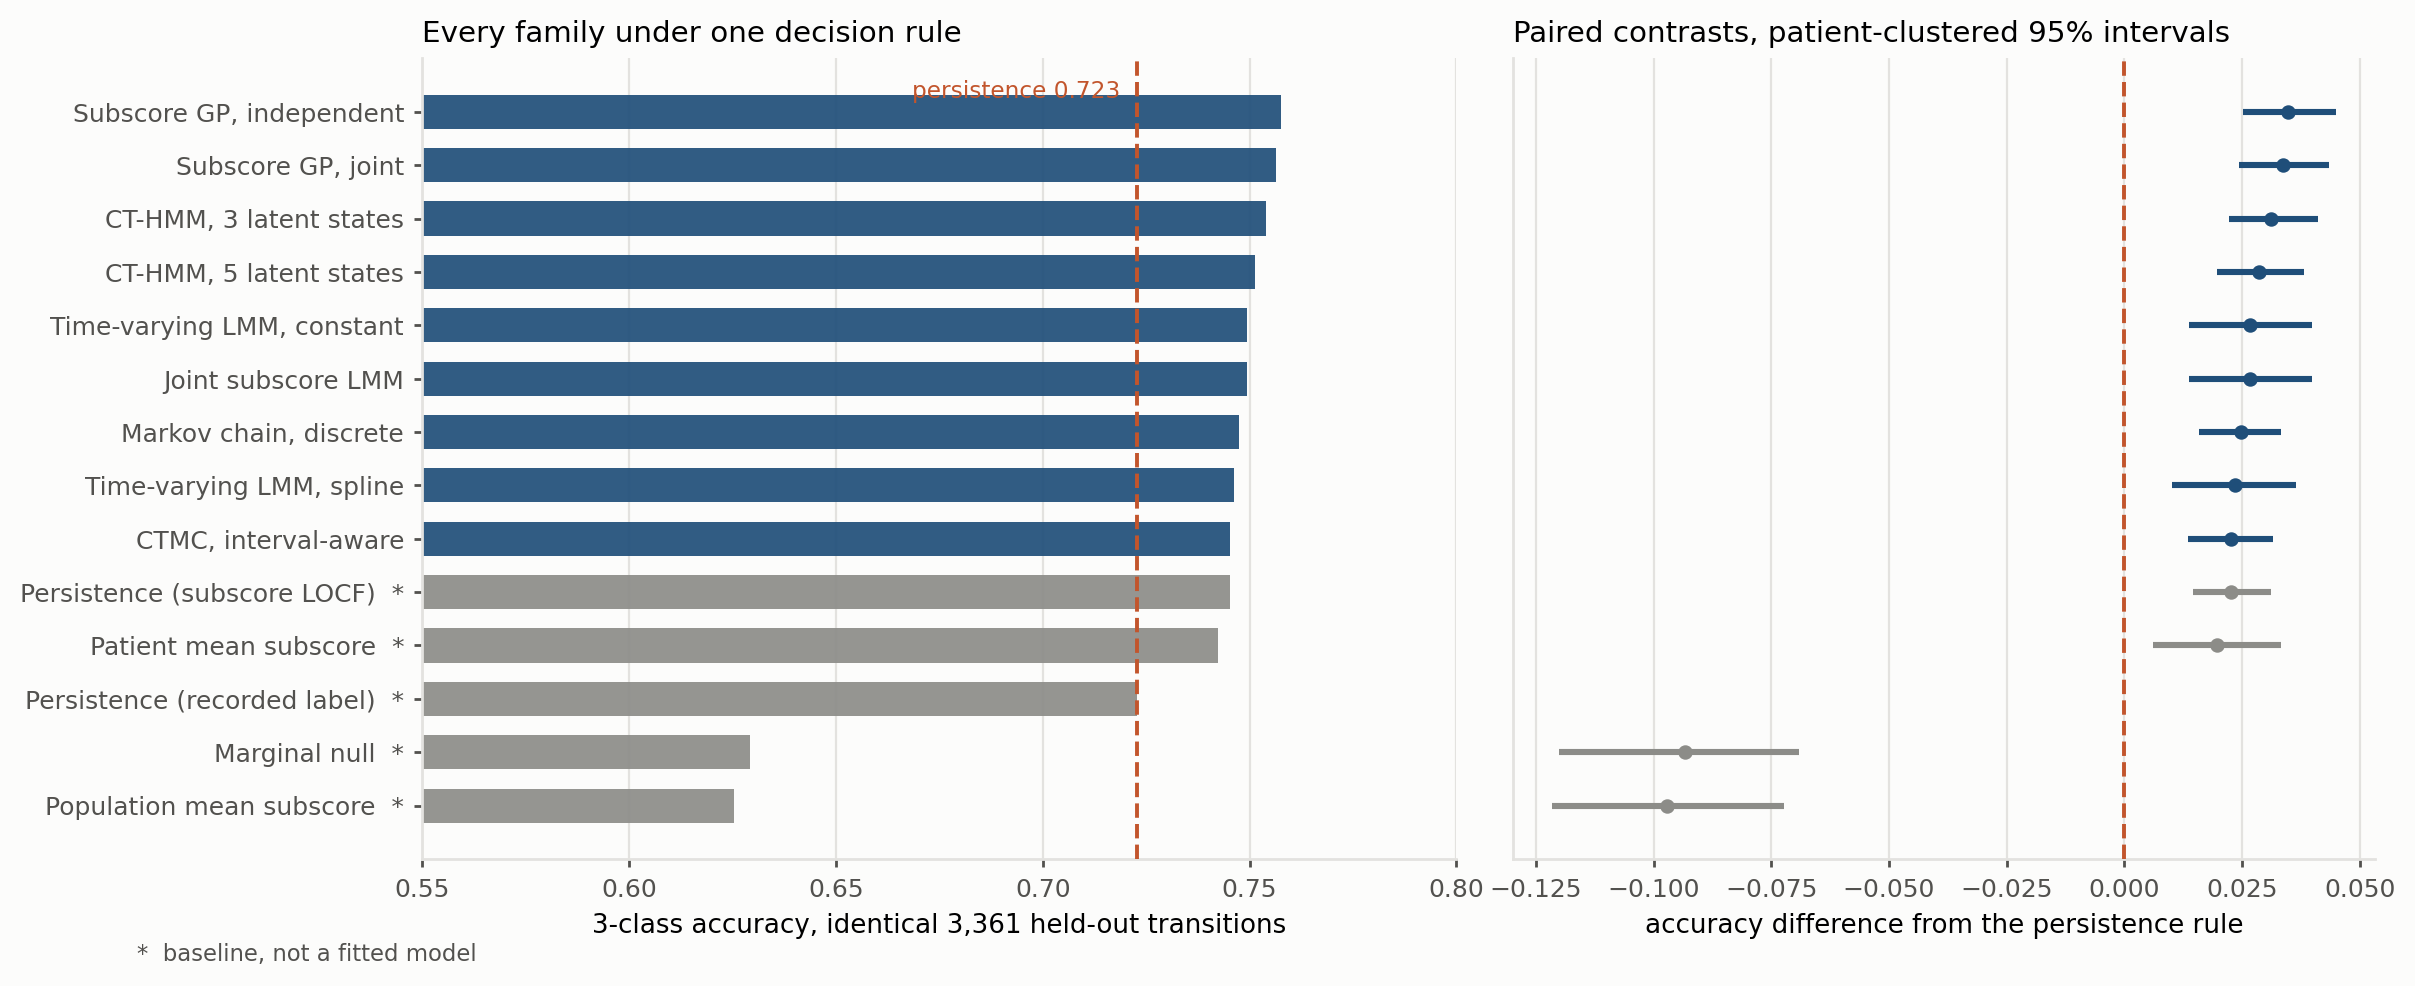
\includegraphics[width=\textwidth]{fig4_families.png}
\caption{Every specification under one decision rule on the identical 3,361
held-out transitions. \textbf{Left:} three-class accuracy; fitted models in
dark, baselines in grey, with the persistence rule marked. The $x$-axis is
truncated at 0.55. \textbf{Right:} the paired accuracy difference of each
specification from the persistence rule, with patient-clustered bootstrap 95\%
intervals. Every fitted specification exceeds persistence and every interval
excludes zero, but the spread between fitted specifications is smaller than the
width of any one interval. Panel labels follow the source analysis: CT-HMM is
the continuous-time hidden Markov model of Section~\ref{sec:hmm} and CTMC the
continuous-time Markov chain of~\eqref{eq:ctmc}. Numerical values are in
Table~\ref{tab:families}.}
\label{fig:families}
\end{figure}

\begin{table}[t]
\centering
\caption{Harmonised comparison of all specifications on the same 3,361 held-out
transitions from 934 patients, under one decision rule (argmax of the three-class
probability vector). ``Rec.\ Ind.'' is recall on the 332 Indeterminate outcomes.
Paired differences against the persistence rule use a patient-level cluster
bootstrap. $^{*}$The five-state hidden Markov model converged in only 404 of 934
folds and is not a like-for-like estimate. $^{\dagger}$The persistence rule emits
only zero and one, so its log loss is clipped and it cannot be calibrated.}
\label{tab:families}
\scriptsize
\setlength{\tabcolsep}{4.5pt}
\begin{tabular}{@{}llrlrrrr@{}}
\toprule
Specification & Family & Acc. & $\Delta$ vs.\ persistence (95\% CI) & Brier & Log loss & Macro-F1 & Rec.\ Ind. \\
\midrule
\multicolumn{8}{@{}l}{\textit{Fitted models}}\\
Subscore GP, independent   & GP               & 0.7575 & $+0.0348$ \,(0.0252, 0.0450) & 0.3602 & 0.6537 & 0.5074 & 0.000 \\
Subscore GP, joint         & GP               & 0.7563 & $+0.0336$ \,(0.0243, 0.0436) & 0.3594 & 0.6518 & 0.5070 & 0.000 \\
HMM, 3 latent states       & latent HMM       & 0.7539 & $+0.0312$ \,(0.0223, 0.0411) & 0.3688 & 0.6726 & 0.5037 & 0.000 \\
HMM, 5 latent states$^{*}$ & latent HMM       & 0.7513 & $+0.0286$ \,(0.0196, 0.0381) & 0.3700 & 0.6746 & 0.5011 & 0.000 \\
Time-varying LMM, constant & mixed model      & 0.7495 & $+0.0268$ \,(0.0136, 0.0398) & 0.3826 & 0.6919 & 0.4977 & 0.000 \\
Joint subscore LMM         & mixed model      & 0.7495 & $+0.0268$ \,(0.0136, 0.0398) & 0.3826 & 0.6919 & 0.4977 & 0.000 \\
Markov chain, discrete     & observed-label   & 0.7474 & $+0.0247$ \,(0.0159, 0.0334) & 0.3896 & 0.7066 & 0.4929 & 0.000 \\
Time-varying LMM, spline   & mixed model      & 0.7462 & $+0.0235$ \,(0.0102, 0.0364) & 0.3794 & 0.6860 & 0.4937 & 0.000 \\
Markov chain, continuous   & observed-label   & 0.7453 & $+0.0226$ \,(0.0135, 0.0316) & 0.3925 & 0.7105 & 0.4909 & 0.000 \\
\addlinespace[3pt]
\multicolumn{8}{@{}l}{\textit{Baselines}}\\
Subscore LOCF              & baseline         & 0.7453 & $+0.0226$ \,(0.0146, 0.0311) & 0.3723 & 0.7556 & 0.4970 & 0.000 \\
Patient-mean subscore      & baseline         & 0.7423 & $+0.0196$ \,(0.0061, 0.0332) & 0.3802 & 0.7594 & 0.4903 & 0.003 \\
\textbf{Persistence}       & \textbf{baseline}& \textbf{0.7227} & ---                   & 0.5546 & 7.6620$^{\dagger}$ & \textbf{0.5559} & \textbf{0.193} \\
Marginal null              & baseline         & 0.6293 & $-0.0934$ \,($-0.1202$, $-0.0691$) & 0.5211 & 0.8756 & 0.2575 & 0.000 \\
Population-mean subscore   & baseline         & 0.6254 & $-0.0973$ \,($-0.1215$, $-0.0723$) & 0.5174 & 0.8716 & 0.3460 & 0.000 \\
\bottomrule
\end{tabular}

\end{table}

\paragraph{Where the margin over the trivial rule comes from.}
Stratifying the comparison by the label recorded at the prediction point
localises the entire effect (Figure~\ref{fig:margin}). For the three-state
hidden Markov model, \textbf{94.3\% of its advantage over persistence comes from
the 334 transitions (9.9\% of the data) at which the current label was
Indeterminate}. Where the current label was TD it gained six correct predictions
out of 2,261; where the current label was PIGD it gained \textbf{none at all}
out of 766, the two rules achieving identical accuracy of 0.7023 on that
stratum. The two approaches made the same call on 98.4\% of current-TD and
96.9\% of current-PIGD transitions, against 0.3\% where the current label was
Indeterminate. The discrete Markov chain makes the point more starkly: it
predicted exactly what persistence predicted on 100\% of both outer strata and
took all 83 of its gained cases from the Indeterminate band.

The fitted models, in other words, did not predict progression better than the
trivial rule. They declined to repeat a class that is rarely repeated, and that
accounts for essentially all of their advantage.

\begin{figure}[t]
\centering
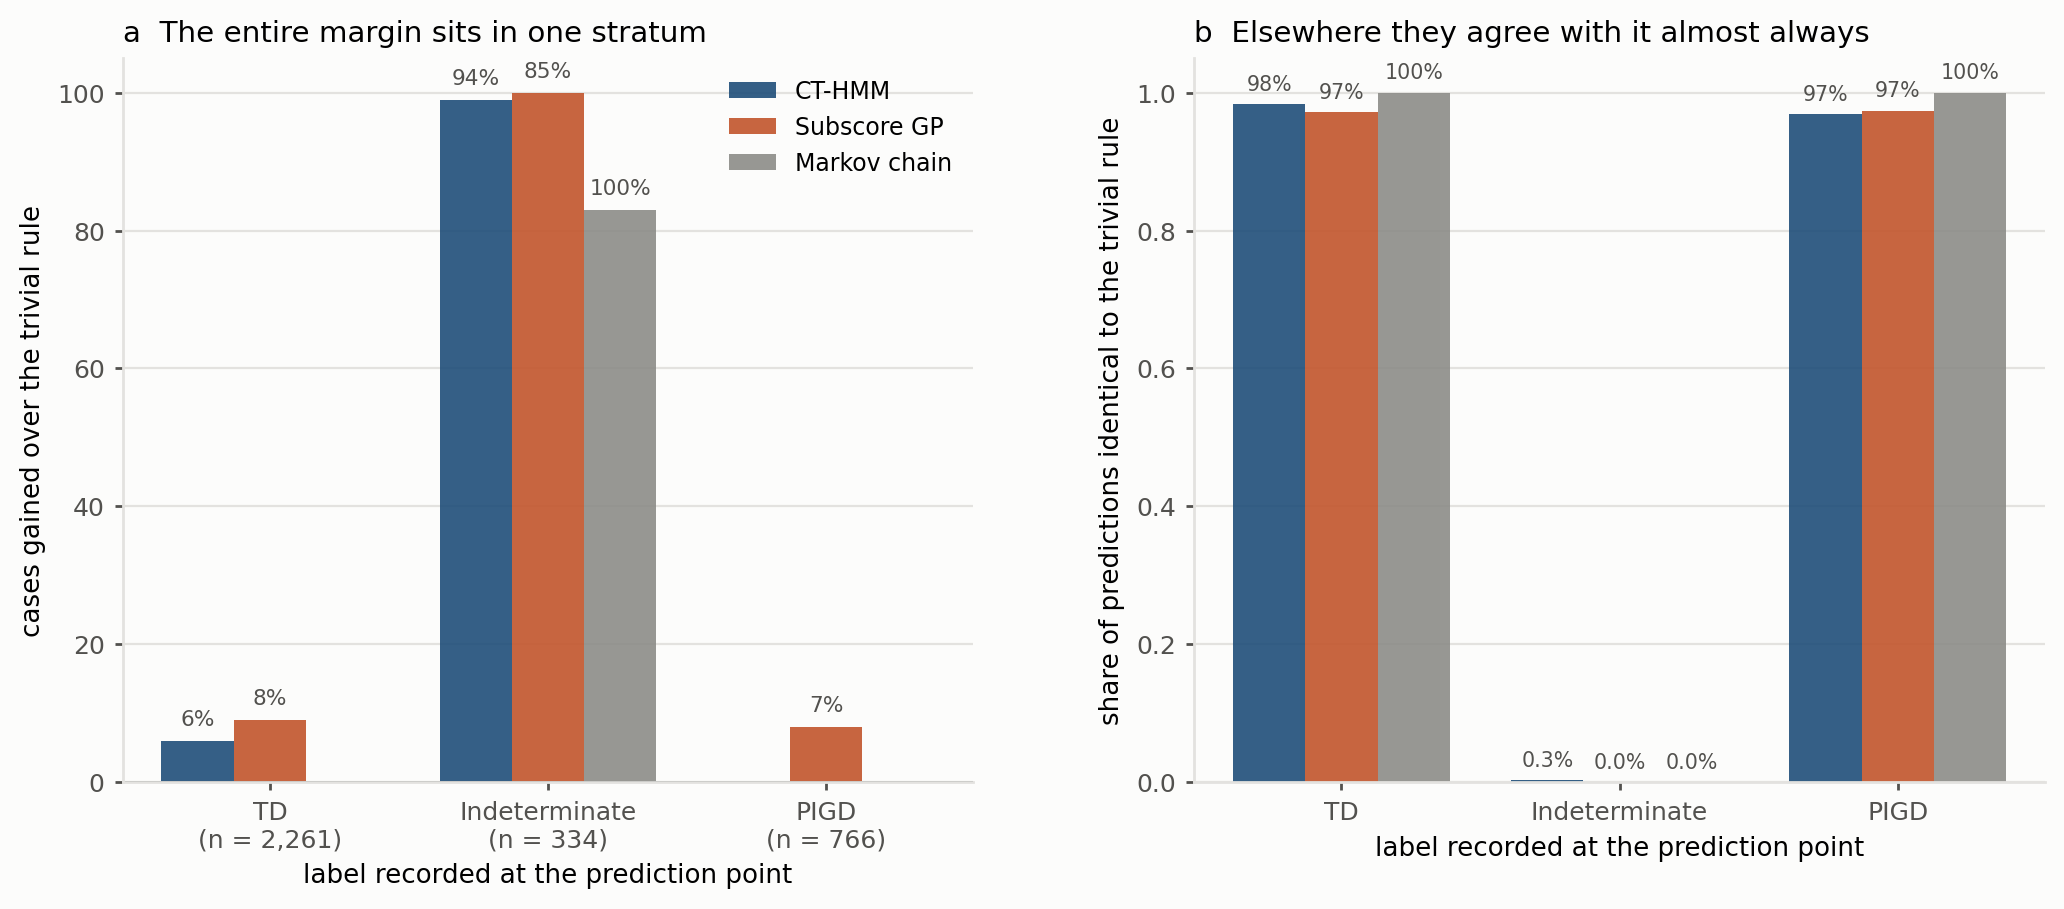
\includegraphics[width=\textwidth]{fig5_margin.png}
\caption{Where each model's advantage over the persistence rule comes from,
decomposed by the subtype recorded at the prediction point. (\textbf{a}) Extra
correct predictions over persistence in each stratum; the percentage above each
bar is that stratum's share of the model's total gain. The Indeterminate
stratum is 9.9\% of the data and supplies 94\% of the hidden Markov model's gain
and 100\% of the discrete chain's. (\textbf{b}) Share of predictions identical
to persistence in each stratum. Outside the Indeterminate band the fitted models
reproduce the trivial rule almost exactly. Panel labels follow the source
analysis: CT-HMM is the three-state hidden Markov model, Subscore GP the
independent subscore Gaussian process, and Markov chain the discrete-time
chain.}
\label{fig:margin}
\end{figure}

\subsection{No model recovers the Indeterminate class, and the band explains why}
\label{sec:ind}

Of the 332 Indeterminate outcomes in the evaluation set, the fitted
specifications recovered essentially none: each predicted the class between zero
and four times in 3,361 opportunities, and per-class recall on Indeterminate was
0.000 for every fitted specification (Table~\ref{tab:families}). Only the
persistence rule predicted it with any frequency --- 334 times, recovering
19.3\% of the Indeterminate outcomes --- and in consequence \textbf{the
persistence rule attains the highest macro-F1 of any specification tested}
(0.5559 against 0.5074 for the best fitted model) while having the lowest
accuracy. Accuracy and macro-F1 rank the specifications in opposite orders here,
because accuracy rewards abandoning a small middle class and macro-F1 does not.

Two measured properties of the band account for this, and neither requires
fitting anything.

\paragraph{The band is narrower than the measurement resolution.}
Because $T$ is a mean of eleven integer ratings and $P$ a mean of five, few
ratio values are attainable inside a band 0.25 wide. The 381 Indeterminate
visits with a defined ratio take only \textbf{eleven distinct values}, of which
198 (52.0\%) sit at $r = 0.9091$ and 100 (26.2\%) at $r = 1.1364$ --- one
hundredth and seven thousandths from a threshold respectively
(Figure~\ref{fig:attainable}). Rebuilding the whole panel under a perturbed rule
that moves both thresholds by less than this spacing (PIGD if $r < 0.91$, TD if
$r > 1.13$) relabels \textbf{298 of 4,441 labelled visits (6.7\%), every one of
them out of the Indeterminate class}. No TD or PIGD visit moves. The
Indeterminate class falls from 441 visits to 143, a reduction of 67.6\%, with
198 becoming PIGD and 100 becoming TD --- exactly the two ratio values above, so
the entire effect is two attainable values crossing a line that moved by 0.01
and 0.0064. Measured over patients rather than visits, the perturbation touches
\textbf{235 of 1,080 (21.8\%)}. This is a deterministic recomputation on a fixed
panel rather than an estimate from a sample, so no uncertainty interval is
reported and none would be appropriate; neither rule is treated as correct.

\begin{figure}[t]
\centering
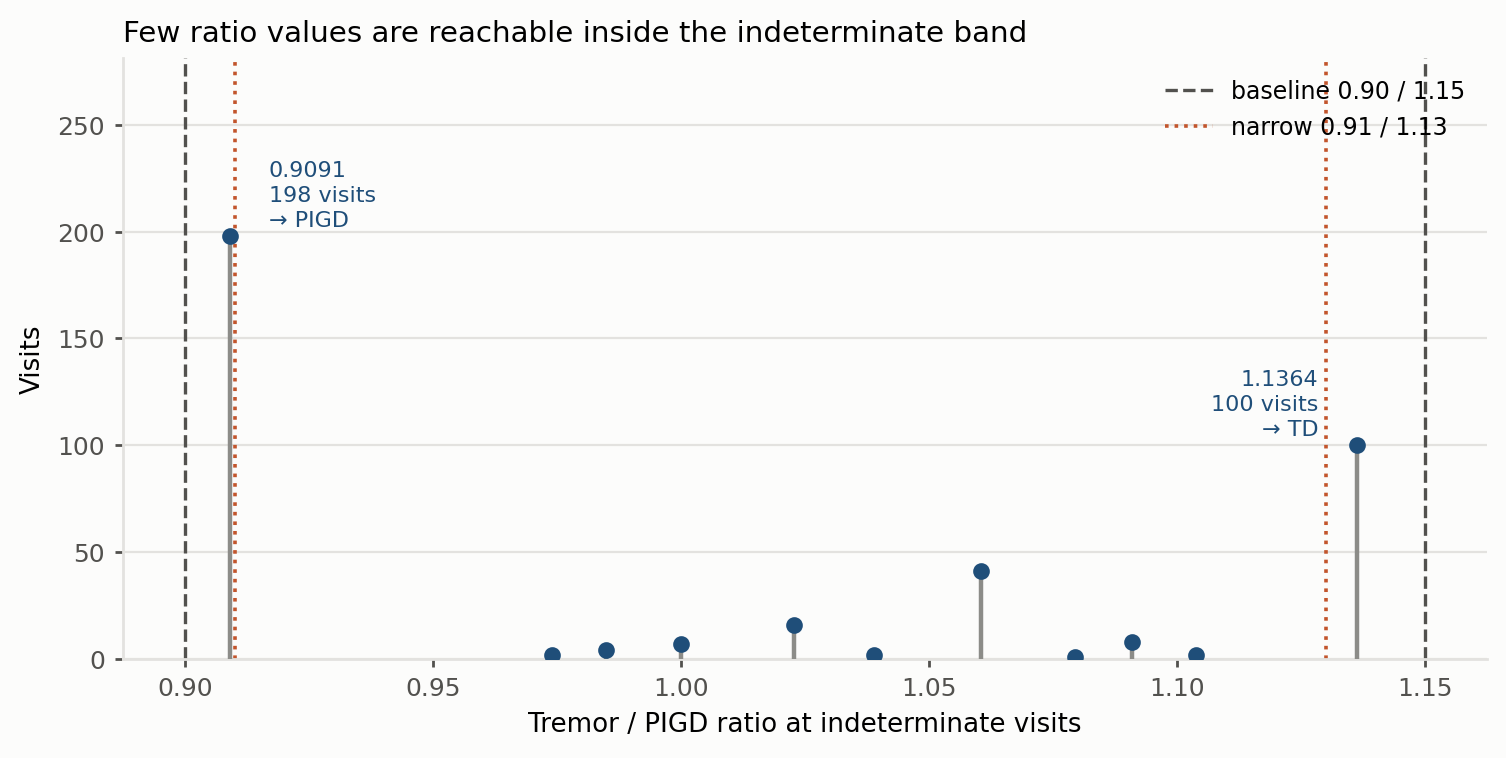
\includegraphics[width=0.88\textwidth]{fig3_attainable.png}
\caption{Attainable values of the ratio inside the Indeterminate band. Each
point is one attainable value of $r = T/P$ and its height the number of
labelled visits taking it; dashed lines are the thresholds of~\eqref{eq:rule}
and dotted lines a perturbation of 0.01 and 0.0064. Of the 381 Indeterminate
visits with a defined ratio, 78\% sit at the two values nearest the thresholds,
and moving the thresholds by less than the spacing of the lattice moves both
values across.}
\label{fig:attainable}
\end{figure}

\paragraph{The residual spread of the underlying quantity dwarfs the band.}
The hierarchical Bayesian growth model (Section~\ref{sec:hbres}) estimates a
total residual SD of $\sigma = 1.14$ for the ratio against an Indeterminate band
$0.25$ wide, a factor of about \textbf{4.6}. A model predicting which of three
bands the next ratio falls in must therefore place a predictive distribution
several times wider than the middle band. Even a perfectly estimated trajectory
would place the next observation almost anywhere relative to that band, so under
an argmax decision rule the middle class is almost never the most probable
outcome. The failure to recover the Indeterminate class is in this sense a
consequence of the representation rather than of any model's capacity.

We note what this does \emph{not} show. These are statements about predicting a
ratio-defined band from a continuous quantity under a particular decision rule.
They do not show that the Indeterminate category is clinically meaningless, and
a decision rule that penalised abandoning the minority class --- or a different
representation of the same examination --- could behave differently. The
macro-F1 column of Table~\ref{tab:families} is the evidence for the first of
those possibilities.

\subsection{Hierarchical Bayesian growth model}
\label{sec:hbres}

Fitted on 2,426 observations from 573 training patients at which the ratio is
defined, the growth model estimates a \textbf{population trend of $-0.0927$ per
year} in the ratio, with a 95\% credible interval of $-0.1159$ to $-0.0682$
(Table~\ref{tab:hb}, Figure~\ref{fig:growth}). The posterior probability that
the population slope is negative is 1.000. On the clinical scale this is a slow
drift of the cohort average away from tremor dominance and towards PIGD.

\begin{table}[t]
\centering
\caption{Posterior summary of the hierarchical Bayesian growth model
of~\eqref{eq:hb}, fitted to 2,426 ratio observations from 573 training patients.
Intervals are 95\% credible intervals.}
\label{tab:hb}
\small
\begin{tabular}{@{}llr@{\hskip 10pt}r@{\,}c@{\,}r@{}}
\toprule
Parameter & Interpretation & Mean & \multicolumn{3}{c}{95\% CrI} \\
\midrule
$\beta_0$ & population baseline ratio              & 2.2920  & ($\phantom{-}$2.1577, & & $\phantom{-}$2.4272) \\
$\beta_1$ & population change in $r$, per year     & $-0.0927$ & ($-0.1159$, & & $-0.0682$) \\
$\sigma$  & total residual SD                      & 1.1380  & ($\phantom{-}$1.0993, & & $\phantom{-}$1.1778) \\
$\tau_0$  & between-patient SD of intercepts       & 1.3408  & ($\phantom{-}$1.2466, & & $\phantom{-}$1.4421) \\
$\tau_1$  & between-patient SD of slopes, per year & 0.1033  & ($\phantom{-}$0.0780, & & $\phantom{-}$0.1315) \\
\bottomrule
\end{tabular}

\end{table}

\begin{figure}[t]
\centering
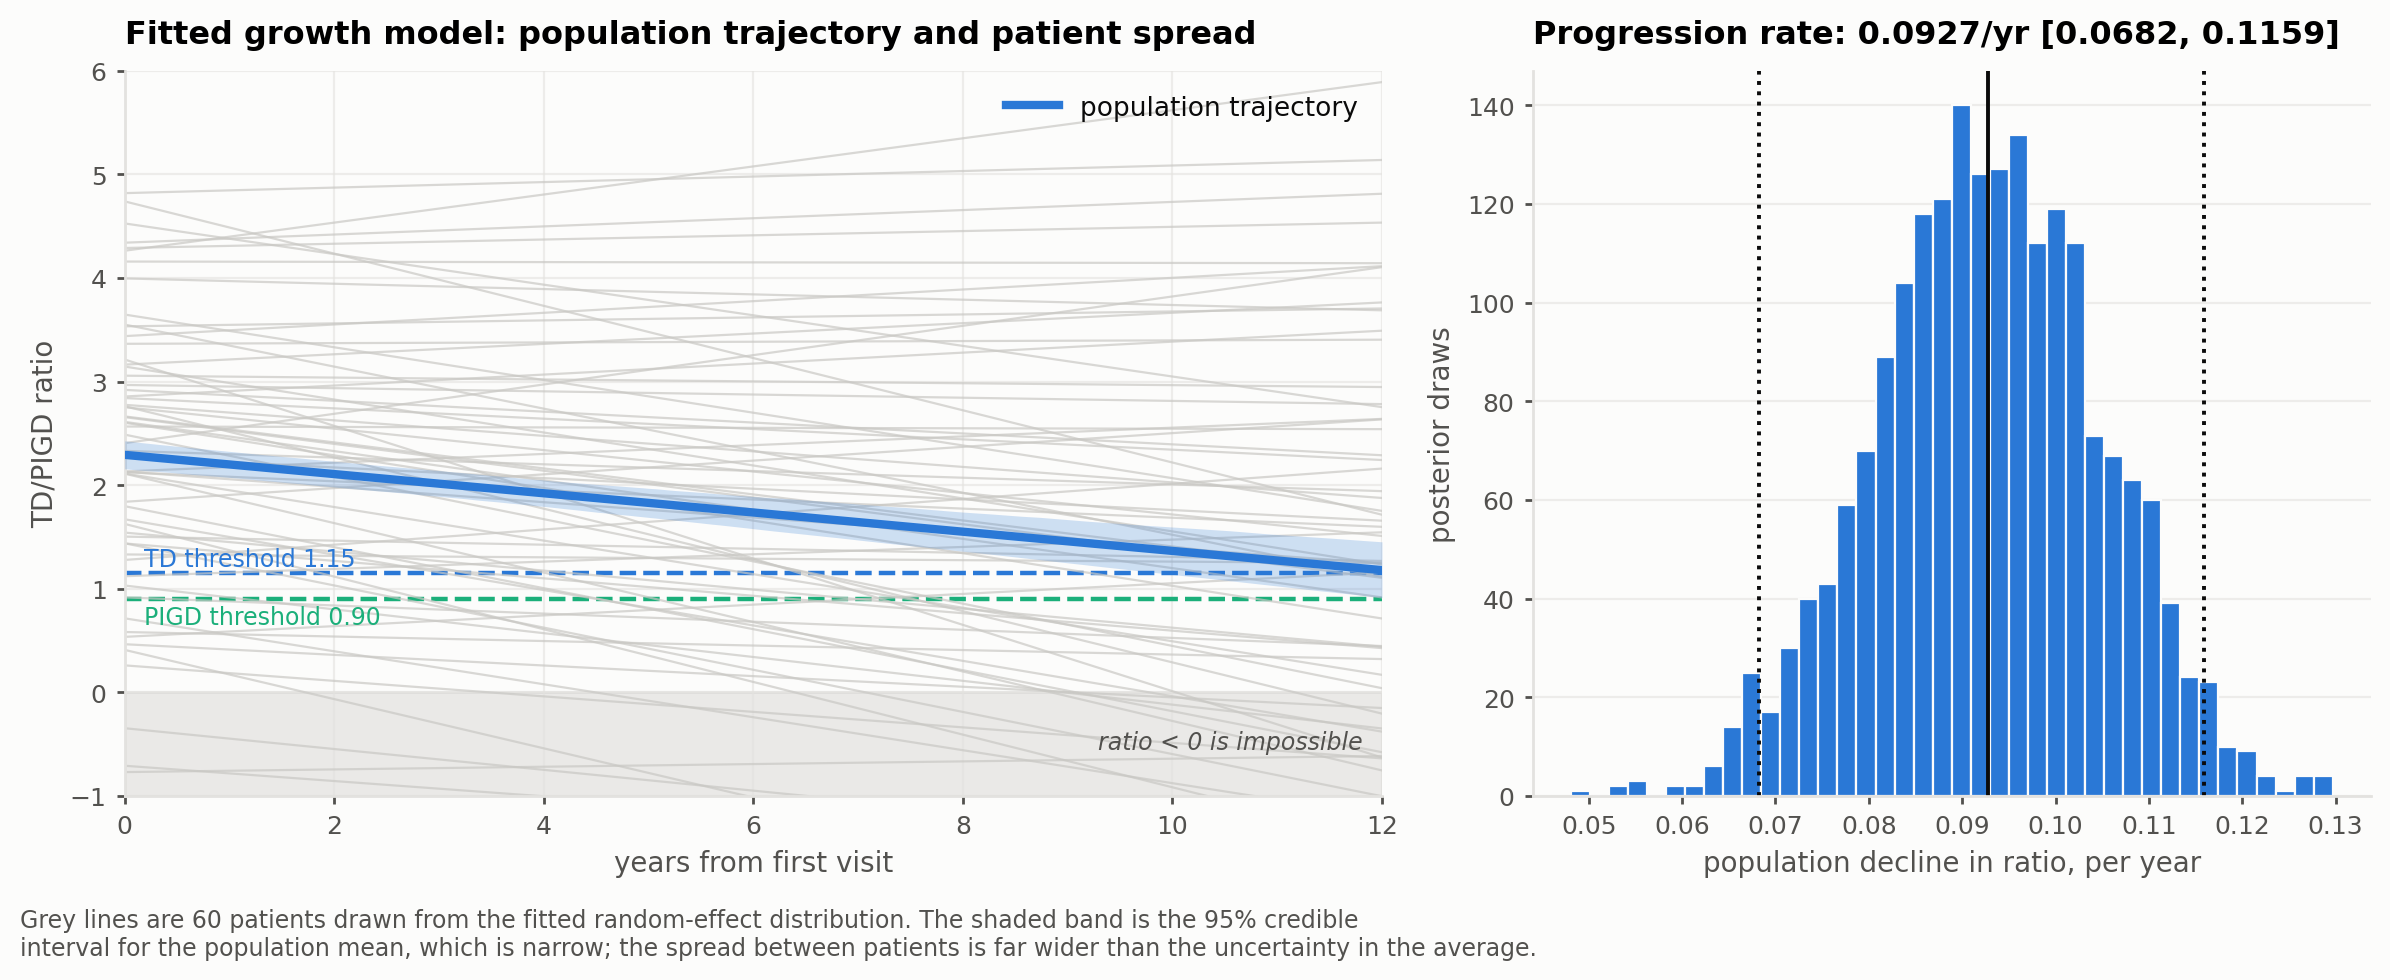
\includegraphics[width=\textwidth]{fig6_growth.png}
\caption{Hierarchical Bayesian growth model of the ratio. \textbf{Left:} the
fitted population trajectory (heavy line) with its 95\% credible band, against
60 patient trajectories drawn from the fitted random-effect distribution (grey);
the two classification thresholds are marked. The credible band on the
population mean is narrow while the spread between patients is wide, so the
population trend is not a patient-level progression rate. The shaded region
below zero marks ratio values that cannot occur, on which the Gaussian
likelihood nonetheless places mass. \textbf{Right:} the posterior for the
population rate of decline, with its median and 95\% credible interval.}
\label{fig:growth}
\end{figure}

Three features of the posterior matter more than the trend itself.

First, \textbf{the population trend is not a patient-level progression rate}.
The between-patient SD of slopes is $\tau_1 = 0.103$ per year, comparable in
magnitude to the population slope of $-0.093$ itself, so the fitted distribution
of individual slopes spans both signs. The credible interval in
Table~\ref{tab:hb} is an interval on the \emph{cohort average}, and
Figure~\ref{fig:growth} shows how much wider the spread of individual
trajectories is than the uncertainty in that average. A statement about the
population here licenses no statement about an individual patient.

Second, \textbf{the residual spread dwarfs the Indeterminate band}. The total
residual SD is $\sigma = 1.138$ (1.099--1.178) against a band 0.25 wide --- the
factor of 4.6 used in Section~\ref{sec:ind}. This is the quantitative form of
the claim that the middle class is nearly unreachable from a continuous
representation under this rule.

Third, on prediction of the next recorded label the growth model does not
improve on the latent-state model. Compared on the same 825 held-out transitions
that both can score --- those where every visit involved has a defined ratio ---
the hidden Markov model reached a held-out log-likelihood of $-0.656$ per
transition against the growth model's $-0.681$, with accuracies of 0.761 and
0.737 and Brier scores of 0.357 and 0.379. Repeating the comparison on six
independent patient-level splits, the hidden Markov model was ahead in 6 of 6,
by a mean of $+0.058$ log-likelihood per transition (SD 0.019; paired
$t$-test $p = 6.6 \times 10^{-4}$, Wilcoxon $p = 0.031$). The growth model's
contribution is therefore an interpretable population trend with uncertainty and
a per-patient slope distribution --- quantities the Markov models do not provide
--- rather than better prediction of the label.

\subsection{Gaussian process models}
\label{sec:gpres}

\paragraph{On the ratio, a flexible kernel helps.}
On one-step-ahead prediction of the ratio (821 patients, 2,707 held-out points
at which the ratio is defined), the squared-exponential kernel $K_1$ reached a
pooled MAE of 0.972 against 1.005 for the linear-trend kernel $K_0$
(Table~\ref{tab:gp}, Figure~\ref{fig:gpr}). The paired difference is
\textbf{$-0.033$ (95\% CI $-0.047$ to $-0.021$)}, and the same sign and
significance hold when errors are averaged within patients before pooling
($-0.019$, $-0.028$ to $-0.011$). Departures from a straight line therefore
carry predictive signal on this quantity.

The remaining kernel contrasts were inconclusive or null. Adding a linear term
beside an RBF changed MAE by about $10^{-6}$, and its variance pinned at its
lower bound in every fold; a Matérn-3/2 kernel did not improve on the squared
exponential ($-0.0005$, $-0.0015$ to $+0.0005$). The linear-kernel Gaussian
process and the hierarchical Bayesian growth model --- two different
implementations of the same linear-trend assumption --- were also
indistinguishable ($-0.0009$, $-0.0033$ to $+0.0014$), which is a useful
internal consistency check rather than a finding.

\begin{table}[t]
\centering
\caption{Gaussian process results. (\textbf{a}) One-step-ahead prediction of the
ratio, leave-one-patient-out. (\textbf{b}) Paired kernel and baseline contrasts
on the ratio; negative values favour the first-named specification, since the
metric is MAE. (\textbf{c}) Paired contrasts on the two subscores, modelled
separately on the full evaluation set. All intervals are patient-clustered
bootstraps.}
\label{tab:gp}
\small
\setlength{\tabcolsep}{5pt}
\begin{tabular}{@{}llrrrr@{}}
\toprule
Target & Specification & MAE & RMSE & CRPS & Cov.\ 95\% \\
\midrule
\multicolumn{6}{@{}l}{\textit{(a) Ratio $r$; 821 patients, 2,707 held-out points}}\\
 & GP, linear kernel ($K_0$)              & 1.005 & 1.387 & 0.747 & 0.939 \\
 & GP, RBF kernel ($K_1$)                 & \textbf{0.972} & 1.357 & 0.725 & 0.941 \\
 & GP, linear $+$ RBF ($K_2$)             & 0.972 & 1.357 & 0.725 & 0.941 \\
 & GP, linear $+$ Mat\'ern-3/2 ($K_3$)    & 0.971 & 1.356 & 0.725 & 0.941 \\
 & Hierarchical Bayesian growth model     & 1.006 & 1.391 & 0.748 & 0.930 \\
 & Persistence                            & 1.043 & 1.540 & 0.818 & 0.936 \\
 & Patient mean                           & 1.063 & 1.471 & 0.800 & 0.941 \\
 & Population mean                        & 1.395 & 1.801 & 0.984 & 0.948 \\
\addlinespace[4pt]
\multicolumn{6}{@{}l}{\textit{(b) Paired contrasts on the ratio (patient-clustered bootstrap)}}\\
\multicolumn{2}{@{}l}{$K_1 - K_0$: does a flexible kernel beat a linear trend?}
   & \multicolumn{4}{l}{$-0.0333$ \,($-0.0467$, $-0.0205$)\quad \textbf{favours $K_1$}} \\
\multicolumn{2}{@{}l}{$K_3 - K_1$: does Mat\'ern beat squared exponential?}
   & \multicolumn{4}{l}{$-0.0005$ \,($-0.0015$, $+0.0005$)\quad inconclusive} \\
\multicolumn{2}{@{}l}{$K_0 - $ growth model: do they agree?}
   & \multicolumn{4}{l}{$-0.0009$ \,($-0.0033$, $+0.0014$)\quad inconclusive} \\
\multicolumn{2}{@{}l}{$K_1 - $ persistence}
   & \multicolumn{4}{l}{$-0.0707$ \,($-0.0979$, $-0.0451$)\quad \textbf{favours $K_1$}} \\
\addlinespace[4pt]
\multicolumn{6}{@{}l}{\textit{(c) Subscores; 934 patients, 3,361 held-out points}}\\
\multicolumn{2}{@{}l}{Tremor subscore: GP $-$ persistence}
   & \multicolumn{4}{l}{$-0.0031$ \,($-0.0084$, $+0.0022$)\quad inconclusive} \\
\multicolumn{2}{@{}l}{PIGD subscore: GP $-$ persistence}
   & \multicolumn{4}{l}{$+0.0134$ \,($+0.0083$, $+0.0187$)\quad \textbf{favours persistence}} \\
\bottomrule
\end{tabular}

\end{table}

\begin{figure}[t]
\centering
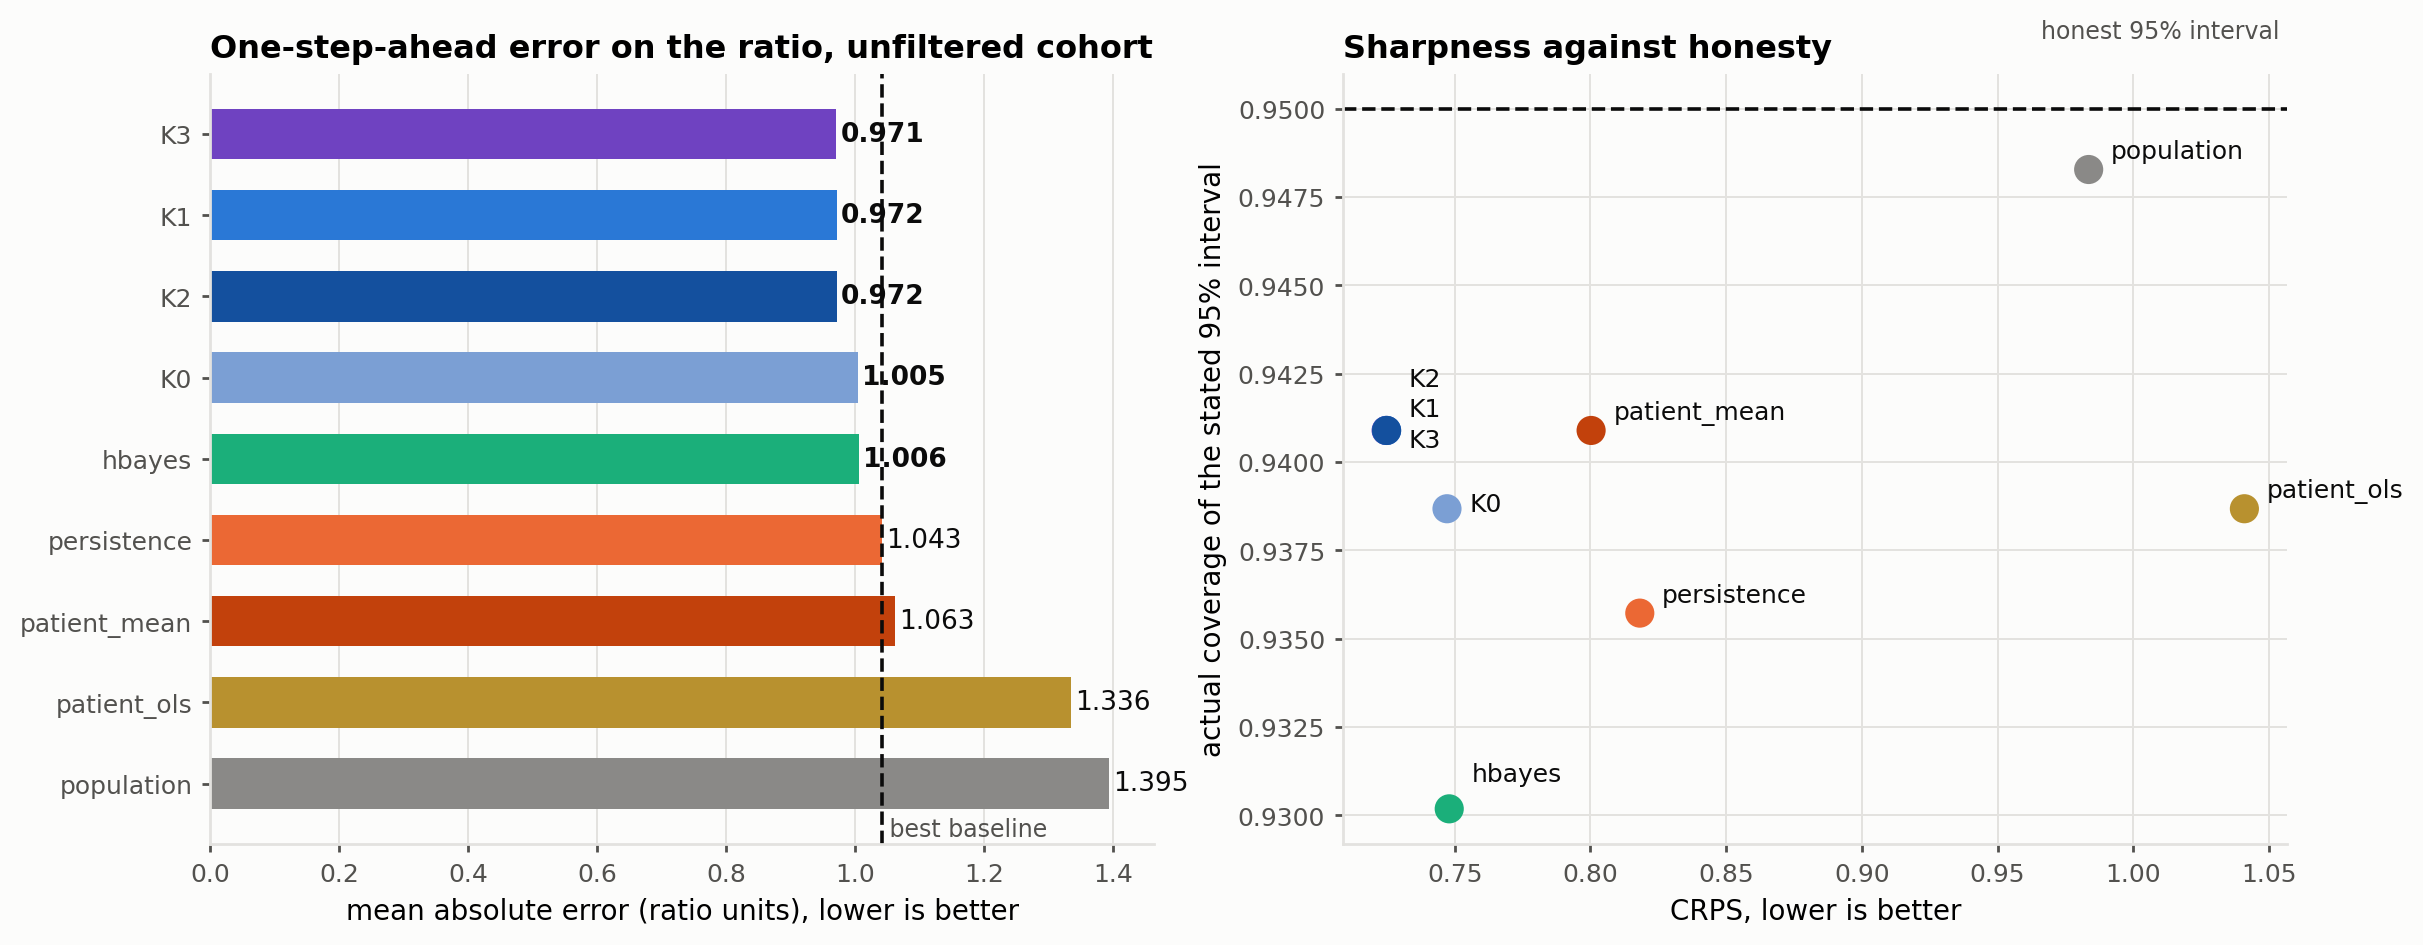
\includegraphics[width=\textwidth]{fig7_gpr.png}
\caption{Gaussian process regression on the ratio, one step ahead and
leave-one-patient-out on 2,707 held-out points. \textbf{Left:} mean absolute
error in ratio units, lower being better, for the four kernels of
Section~\ref{sec:gp}, the hierarchical Bayesian growth model and the rule
baselines; the dashed line marks the best baseline. The RBF kernels ($K_1$,
$K_2$, $K_3$) separate from the linear kernel $K_0$ and from the growth model,
which are themselves indistinguishable from each other. \textbf{Right:}
sharpness against honesty --- CRPS on the $x$-axis against the realised coverage
of the stated 95\% predictive interval on the $y$-axis, with nominal coverage
marked. All specifications are slightly under-covered.}
\label{fig:gpr}
\end{figure}

\paragraph{On the subscores, it does not.}
The advantage does not survive the change of target. Modelled separately on the
full evaluation set of 3,361 points from 934 patients, the Gaussian process
\textbf{did not beat persistence on the tremor subscore} ($-0.0031$, 95\% CI
$-0.0084$ to $+0.0022$; interval contains zero) and was \textbf{worse than
persistence on the PIGD subscore} ($+0.0134$, 95\% CI $+0.0083$ to $+0.0187$;
interval excludes zero, in favour of the trivial rule). The jointly-covarying
form did not change this: the joint and diagonal specifications differed by
$-0.0003$ on tremor and $-0.0001$ on PIGD, both intervals containing zero.

The reason is the point mass at zero. At the 446 held-out visits where the PIGD
subscore is zero, persistence predicts below 0.1 at 62\% of them, while the
Gaussian process never does --- its mean prediction there is 0.242. A continuous
Gaussian model cannot reproduce an exact zero, and a sixth of this cohort's
visits carry one. The same misspecification is visible as predictive mass below
zero: 12.9\% to 13.9\% of each ratio predictive distribution and 5.3\% of the
tremor distribution fall on values the quantity cannot take.

\paragraph{Calibration.}
Coverage of the stated 95\% predictive intervals on the ratio was 0.941 for the
Gaussian processes and 0.930 for the growth model, so all specifications are
slightly under-covered (Figure~\ref{fig:gpr}, right).

\subsection{Matched comparison of the Gaussian process and the hidden Markov model}
\label{sec:matched}

Converting the subscore Gaussian process predictions back to a subtype through
the unchanged rule~\eqref{eq:rule} permits a like-for-like comparison with the
hidden Markov model. The comparison is matched in the strongest sense available
here: \textbf{exactly the same 934 patients and the same 3,361 prediction
points}, with the same target label at every point, the same leave-one-patient-out
protocol, the same decision rule, and a paired bootstrap that shares one
patient-level resample between the two conditions in every replicate.

GP-derived accuracy was \textbf{75.66\%} against the hidden Markov model's
\textbf{75.39\%}, a paired difference of \textbf{$+0.27$ accuracy points (95\%
CI $-0.42$ to $+0.98$)}.\footnote{The same specification appears at 0.7575 in
Table~\ref{tab:families}. The two figures are different Monte Carlo
realisations of the same conversion from the same saved predictive
distributions: Table~\ref{tab:families} uses the draws generated for the
all-specification comparison, and this section uses the draws generated with the
hidden Markov model as the paired comparator. They differ by 0.0009, within the
Monte Carlo error of the conversion, which a half-draw check bounds at 0.0015
(Section~\ref{sec:gp}). The paired contrast here is computed within a single set
of draws and is unaffected.}

The interval contains zero. Two models built on entirely different premises ---
one a latent discrete state observed through a misclassification matrix, the
other a pair of continuous trajectories pushed through a thresholding rule ---
land within a third of an accuracy point of each other on identical data.

\textbf{This is a failure to detect a difference, not a demonstration of
equivalence.} The interval is roughly $1.4$ accuracy points wide, so differences
smaller than about one point are not resolvable at this sample size, and no
equivalence margin was specified in advance. The two models also differ on
quantities this comparison does not measure: they produce different probability
vectors, the Gaussian process additionally predicts the subscores themselves,
and the hidden Markov model requires no subscores at prediction time.

\subsection{Summary of findings}

Taken together, the results across the four families are consistent on four
points.

\emph{Model complexity does not materially change predictive performance on this
target.} Four families embodying substantially different assumptions --- a chain
in the recorded label, a latent state observed through a misclassification
matrix, a parametric growth model on the ratio, and non-parametric trajectories
on the subscores --- land within 1.22 accuracy points of one another on one case
list, and the best of them is $+3.1$ points above a rule with no parameters.
Within the discrete-state family, raising the latent state count from three to
five did not help, and the larger specification did not reliably fit.

\emph{The convergence carries more weight than any single accuracy figure.}
Agreement between families that disagree about what generates the data is
evidence about the data, not about a modelling choice.

\emph{The Indeterminate class is not recovered by anything fitted.} Its recall
is zero for every fitted specification, the trivial rule attains the best
macro-F1 by virtue of being the only one that predicts the class at all, and two
independently measured properties of the band --- the lattice of attainable
ratios and a residual spread 4.6 times the band width --- account for this
without reference to model capacity.

\emph{Label reliability bounds what the comparison can mean.} The target changes
frequently, a third of those changes are undone at the next assessment, the
estimated conversion incidence halves under a sustained-change definition, and
the recorded label is not first-order Markov. These are properties of the
endpoint, measurable before any model is fitted, and each of them constrains what
any model trained on it could achieve.

% =====================================================================
\section{Discussion}
% =====================================================================

\subsection{Principal interpretation}
On one cohort and one evaluation protocol, four dissimilar model families
predicted the next recorded motor subtype within 1.22 accuracy points of one
another, with the best gaining about three points over a rule that repeats the
current label. Essentially all of that shared advantage arose on the one tenth
of assessments recorded Indeterminate, and none of the fitted models recovered
that class. Over the same transitions, more than a third of observed subtype
changes were reversed at the following visit, and moving the decision thresholds
by less than the spacing of attainable ratio values relabelled a fifth of
patients.

Read together, these results locate the limit on longitudinal subtype prediction
in this cohort in the reliability and representation of the label rather than in
the capacity of the models. That is a claim about this target, in this cohort,
under this protocol. It is not a claim that model capacity is irrelevant in
general, and it is not a claim that the families compared here exhaust what
could be tried.

\subsection{Why model capacity may not be the binding constraint}
The argument rests on convergence rather than on any one number. Markov chains
in the observed label, a hidden Markov model with an explicit misclassification
matrix~\citep{jackson2011}, a hierarchical Bayesian growth model and Gaussian
processes on the subscores~\citep{rasmussen2006} embody different assumptions
about what generates the data: whether there is a latent state at all, whether
the quantity of interest is discrete or continuous, whether trajectories are
linear, and whether the elapsed interval matters. Agreement among specifications
that disagree this much is more naturally read as a property of the data than as
a coincidence of modelling choices.

The construction of the target supports the same reading. The subtype is a
deterministic threshold on a ratio of two means, so predicting it reduces to
predicting where that ratio will fall relative to two cut points. When the
predictive spread of the ratio is several times the width of the middle band,
and when the attainable values inside that band cluster at its edges, the
achievable accuracy is largely fixed by the arithmetic of the rule and the noise
in the ratings, not by the flexibility of the function class.

Two limits on this argument should be stated plainly. First, four families are
not all families; a representation of the same examination that we did not try
could behave differently, and Section~\ref{sec:future} describes one we are
pursuing. Second, the harmonised comparison standardises \emph{evaluation}, not
\emph{estimation}: families were fitted under their own schemes, so a difference
in fitting efficiency would appear here as a difference in accuracy and could not
be separated from a difference in capacity.

\subsection{What the Indeterminate class is}
The results are most naturally read as saying that, as operationalised, the
Indeterminate band behaves like the neutral zone of a noisy continuous quantity
rather than like a third state. It was the least persistent recorded state by a
wide margin (0.192), it was the origin and destination of the changes most
likely to reverse, and it is where every fitted model found its advantage --- not
by predicting it, since none did at any useful rate, but by declining to repeat
a class that is rarely repeated.

Its fragility is arithmetic as much as clinical. Half of Indeterminate visits
with a defined ratio sit at a single attainable value one hundredth from a
threshold, and moving the thresholds by about 0.02 relabels 6.7\% of all
labelled visits and a fifth of patients, every one of them out of that class.
The emission constraint in the latent-state specification was binding for this
state alone, at exactly $E_{aa} = 0.5$, which is the same fact expressed in the
model's parameters.

We draw a narrow conclusion from this. These are measurement-level observations
about a band defined by thresholding a ratio; they do not establish that the
Indeterminate category is clinically meaningless, and they would not transfer
automatically to a differently constructed middle category. Whether the PIGD
construct identifies a distinct phenotype has been questioned on clinical
grounds~\citep{nutt2016,urso2022}; our results add a measurement-level reason
for caution that is confined to the Indeterminate category.

\subsection{Interpreting the Gaussian process and hidden Markov model comparison}
\label{sec:interp-matched}
The matched comparison of Section~\ref{sec:matched} connects two different ways
of approaching the same question. The hidden Markov model predicts a discrete
label through a latent discrete state; the Gaussian process predicts two
continuous symptom scores and the label is derived from them afterwards by the
unchanged rule. That these produce accuracies within $0.27$ points of each other
on identical data suggests that the information relevant to the next label is
largely shared between the two representations, and that the step from
continuous symptom prediction to discrete subtype prediction discards much of
what distinguishes them.

Similar accuracy does not make the models equivalent, and we do not claim it
does. The interval on the paired difference contains zero, which at this sample
size rules out differences larger than about one accuracy point but establishes
nothing about smaller ones; no equivalence margin was pre-specified. The two
models differ in their probability vectors, in what they predict besides the
label, and in what they require as input. They also differ in where their errors
fall: the Gaussian process gained a small number of cases in the TD and PIGD
strata where the hidden Markov model gained six and none respectively
(Figure~\ref{fig:margin}a).

\subsection{Clinical implications}
We treat the clinical implications cautiously, because this study does not
establish clinical utility and was not designed to.

What the results do support is a set of recommendations about how the TD/PIGD
label is used as a longitudinal endpoint. A conversion endpoint defined on a
single assessment overstated incidence in this cohort by roughly a factor of two
relative to one requiring a sustained change, so the definition belongs in a
study protocol rather than in the analysis. A pooled transition matrix is an
attendance-weighted average of intervals that behave differently and is not a
property of the disease. And a reported accuracy on this endpoint is close to
uninterpretable without the accuracy of a parameter-free rule on the identical
case list, which here was 0.723.

What the results do \emph{not} support should be equally explicit. This study
does not demonstrate readiness for clinical deployment, does not show improved
patient outcomes, does not validate any clinical diagnosis, does not support any
treatment recommendation, does not establish that any model is clinically
superior to any other, and does not establish generalisation beyond this cohort.

\subsection{Limitations}
\label{sec:limits}

\begin{enumerate}
\itemsep3pt
\item \textbf{The target is a rule's output, not an independent diagnosis.} We
predict the next recorded subtype label, which is a deterministic recomputation
of a published rule on sixteen ratings. The reversion we measure is reversion of
that rule's output and includes both genuine phenotypic fluctuation and rating
variability; this design cannot separate them.

\item \textbf{The ratio is undefined when the PIGD subscore is zero.} This
affects 725 of 4,441 labelled visits (16.3\%), and 692 of the 4,295 visits in
the modelling cohort (16.1\%). Specifications defined on the ratio --- the
growth model and the ratio Gaussian process --- drop these visits entirely.

\item \textbf{The ratio-based subset is not a random subset.} The excluded
visits are overwhelmingly tremor dominant (665 of 725 are TD). Quantities
estimated on the ratio subset are therefore conditioned on the presence of some
postural or gait impairment and are not cohort-wide.

\item \textbf{The Indeterminate class is not predicted by any fitted model.}
Every three-class accuracy reported here is attained while recovering none of
the 332 Indeterminate outcomes, and the persistence rule attains the best
macro-F1 for precisely that reason.

\item \textbf{The matched comparison does not establish equivalence.} Its
interval contains zero at a width of about 1.4 accuracy points, and no
equivalence margin was pre-specified.

\item \textbf{Evaluation was harmonised; estimation was not.} Families were
fitted under their own schemes and their saved predictions were scored under one
protocol, so fitting efficiency and model capacity are not separable in the
comparison.

\item \textbf{Gaussian likelihoods on bounded, non-negative scores.} The ratio
models place 12.9\% to 13.9\% of their predictive mass below zero and the tremor
model 5.3\%, on values those quantities cannot take. No point prediction is
negative, but the misspecification is real and is the subject of
Section~\ref{sec:future}.

\item \textbf{Complete-case analysis with non-random label loss.} 89.6\% of
unlabelled visits lacked an OFF-medication examination, concentrating the loss
in treated patients later in follow-up.

\item \textbf{Conditional on attendance.} Every transition probability is
conditional on the next visit occurring, and every model is given the interval
to that visit, so none addresses when a patient will next be seen.

\item \textbf{Model-specific caveats.} The five-state hidden Markov model
converged in only 404 of 934 folds and is reported as a negative result about
capacity, not as a comparable accuracy estimate. The growth model used a single
Gibbs chain; its half-chain stability was checked but formal multi-chain
convergence diagnostics were not computed. The information criteria favouring
the latent layer assume independent observations and so favour it more than
clustered data warrant.

\item \textbf{One cohort, no external validation.} All results come from the
PPMI sporadic Parkinson's disease cohort. Nothing here has been replicated in an
external cohort, and the study should not be described as externally validated.

\item \textbf{No clinical utility is established.} This is a measurement and
benchmarking study on a derived endpoint.

\item \textbf{Multiplicity and post-hoc analyses.} Multiplicity is largely
uncorrected across the specifications compared, and the margin decomposition,
though computed within a pre-specified protocol, was not an anticipated result
and should be read as a discovery rather than a pre-registered test.
\end{enumerate}

\subsection{Future work}
\label{sec:future}
Three of the limitations above --- the undefined ratio, the systematically
excluded tremor-dominant visits, and the predictive mass placed below zero ---
are the same problem seen from different angles. All follow from modelling a
ratio, or modelling bounded non-negative subscores with a Gaussian likelihood.

Work now in progress models the tremor and PIGD subscores \emph{jointly} under a
\emph{bounded} likelihood, deriving the subtype afterwards through the unchanged
rule~\eqref{eq:rule}. A joint model on the two subscores never forms the ratio,
so visits with $P = 0$ remain in the analysis and the 692 excluded visits of the
modelling cohort are recovered; and a likelihood respecting the bounded,
zero-inflated support of a mean of integer ratings in $[0,4]$ cannot place
predictive mass on impossible values, removing the 5\%--14\% of mass that the
Gaussian specifications place below zero. Whether this changes the prediction of
the recorded label is an open question. The results reported in this paper give
no reason to expect a large change in accuracy, since the limiting factor
identified here is the label and its band rather than the likelihood; the
expected gain is a correctly specified predictive distribution and a cohort that
is no longer conditioned on the presence of gait or postural impairment.

\textbf{This is ongoing work and no result from it is reported here.} It is
described because it addresses limitations of the present study, not as evidence
for any claim made in it.

Two further directions follow from the measurements rather than the models.
Replication in an independent cohort would establish whether the reversion rate
and the band's fragility are properties of this cohort or of the rule.
And because the limiting factor identified here is the categorical endpoint,
the more promising object of study where the question is progression rather than
classification may be a continuous description of the same examination.

% =====================================================================
\section{Conclusion}
% =====================================================================

We asked whether longitudinal prediction of the Parkinson's disease motor
subtype is limited more by model capacity or by the reliability and
representation of the label. In this cohort, under one evaluation protocol, the
evidence points to the label.

Four model families embodying substantially different assumptions --- Markov
chains in the recorded label, a hidden Markov model with a latent state and a
fitted misclassification matrix, a hierarchical Bayesian growth model on the
ratio, and Gaussian processes on the ratio and the subscores --- converged to
within 1.22 accuracy points of one another on 3,361 held-out transitions from
934 patients. The best discrete-state specification exceeded a parameter-free
persistence rule by $+3.1$ accuracy points (95\% CI $+2.2$ to $+4.1$), and
essentially all of that advantage arose on the 9.9\% of assessments recorded
Indeterminate. No fitted model recovered that class. Converting continuous
subscore predictions back through the unchanged classification rule put a
Gaussian process and a hidden Markov model within $0.27$ accuracy points of each
other on identical data, with an interval containing zero.

Against this, the endpoint itself proved unstable: 35.2\% of observed subtype
changes reversed at the very next visit, requiring a conversion to hold for two
consecutive assessments removed 51.7\% of apparent PIGD conversions, the
recorded label failed a first-order Markov test in all three states, and moving
the thresholds by less than the spacing of attainable ratio values relabelled a
fifth of patients. A total residual spread of 1.14 against an Indeterminate band
0.25 wide explains, without reference to any model, why the middle class is not
recovered.

The contribution is a set of measurements about an endpoint and a protocol under
which claims about it can be compared, not a new model. The practical
consequence is not that the TD/PIGD distinction should be discarded, which these
results do not support, but that its use as a longitudinal endpoint should rest
on a sustained-change definition, an interval-aware treatment of follow-up, and
a reported comparison against a trivial rule on the identical case list. Where
the question is progression rather than classification, a continuous
representation of the same examination --- modelled jointly and under a bounded
likelihood, as in the ongoing work described above --- is the more promising
direction.

These conclusions are bounded by the limitations of Section~\ref{sec:limits}.
They concern one observational cohort, one labelling rule, and four model
families; no external cohort was used, no clinical utility is established, and
the comparisons that failed to detect a difference do not establish equivalence.

% =====================================================================
\section*{Data Availability}
% =====================================================================
\addcontentsline{toc}{section}{Data Availability}
Data used in the preparation of this article were obtained from the Parkinson's
Progression Markers Initiative (PPMI) database
(\url{www.ppmi-info.org/access-data-specimens/download-data}). For up-to-date
information on the study, visit \url{www.ppmi-info.org}. PPMI data are available
to qualified researchers under the PPMI Data Use Agreement and cannot be
redistributed by the authors. Analysis code and the configuration fixing every
parameter of the pipeline are maintained in the project repository.

\setlength{\bibsep}{4pt}
\bibliographystyle{plainnat}
\bibliography{refs}

\end{document}
